%% LyX 2.3.2 created this file.  For more info, see http://www.lyx.org/.
%% Do not edit unless you really know what you are doing.
\documentclass{article}
\usepackage[utf8]{inputenc}
\usepackage{geometry}
\geometry{verbose,tmargin=2.5cm,bmargin=2cm,lmargin=2cm,rmargin=2cm}
\usepackage{array}
\usepackage{verbatim}
\usepackage{float}
\usepackage{units}
\usepackage{mathtools}
\usepackage{amsmath}
\usepackage{graphicx}

\makeatletter

%%%%%%%%%%%%%%%%%%%%%%%%%%%%%% LyX specific LaTeX commands.
%% Because html converters don't know tabularnewline
\providecommand{\tabularnewline}{\\}
%% Strike out display math with tikz
\usepackage{tikz}
\usetikzlibrary{calc}
\newcommand{\lyxmathsout}[1]{%
  \tikz[baseline=(math.base)]{
    \node[inner sep=0pt,outer sep=0pt](math){#1};
    \draw($(math.south west)+(2em,.5em)$)--($(math.north east)-(2em,.5em)$);
  }
}

%%%%%%%%%%%%%%%%%%%%%%%%%%%%%% Textclass specific LaTeX commands.
\newcommand{\lyxaddress}[1]{
	\par {\raggedright #1
	\vspace{1.4em}
	\noindent\par}
}

%%%%%%%%%%%%%%%%%%%%%%%%%%%%%% User specified LaTeX commands.
\usepackage{xr}
\externaldocument{Paper_req-550_V1.0.1}
\usepackage{lineno}
\usepackage{xcolor}
\usepackage{tikz}
\usetikzlibrary{arrows}

\newcommand{\bs}[1]{\boldsymbol{#1}}
\newcommand{\add}[1]{\textcolor{red}{#1}}
\newcommand{\oran}{\mathrm{o}}
\newcommand{\g}{\mathrm{g}}
\newcommand{\X}{\mathrm{X}}
\newcommand{\Y}{\mathrm{Y}}
\newcommand{\PP}{\mathrm{P}}
\newcommand{\EE}{\mathrm{E}}
\newcommand{\RR}{\mathrm{RR}}
\newcommand{\DD}{\mathrm{DD}}

\newcommand{\HH}{\mathrm{H}}
\newcommand{\A}{\mathrm{A}}
\newcommand{\I}{\mathrm{I}}
\newcommand{\M}{\mathrm{M}}
\newcommand{\OO}{\mathrm{O}}

\newcommand{\sh}{\mathrm{sh}}
\newcommand{\nullm}{\mathrm{null}}
\newcommand{\intv}{\mathrm{intv}}
\newcommand{\family}{\mathrm{visit}}
\newcommand{\care}{\mathrm{care}}
\newcommand{\Exp}{\mathrm{exp}}
\newcommand{\onset}{\mathrm{onset}}

\makeatother

\begin{document}
\title{Supplementary Methods and Results\\Empowering the crowd: Feasible
strategies \\ to minimize the spread of COVID-19 \\ in informal
settlements}
\author{Alberto Pascual-García$^{(1,*)}$, Jordan Klein$^{(2)}$, Jennifer
Villers$^{(3,\land)}$, \\ Eduard Campillo-Funollet$^{(4,\wedge)}$,
Chamsy Sarkis$^{(5)}$}

\maketitle
\medskip{}


\lyxaddress{\begin{center}
(1) Institute of Integrative Biology. ETH-Zürich. Zürich, Switzerland.
\\ (2) Office of Population Research. Princeton University. Princeton,
NJ, USA. \\ (3) Princeton Environmental Institute. Princeton University.
Princeton, NJ, USA. \\ (4) Genome Damage and Stability Centre. University
of Sussex. Brighton, United Kingdom. \\ (5) Pax Syriana Foundation.
Valetta, Malta. \\ ($\land$) Equal contribution. \\ ({*}) correspondence:
alberto.pascual@env.ethz.ch
\par\end{center}}

\newpage{}

\section*{Parameterization of the model}

\subsection*{Derivation of fixed parameters (Table \ref{tab:FixedParams} in Main
Text)}

To estimate the latent period ($\nicefrac{1}{\delta_{\EE}}$), we
calculated the difference between randomly generated incubation ($\nicefrac{1}{\delta_{\EE}}+\nicefrac{1}{\delta_{\PP}}$)
and presymptomatic ($\nicefrac{1}{\delta_{\PP}}$) periods. We estimated
the presymptomatic period using results reported by He et al. \cite{he2020temporal}
and found they best fit a Gompertz distribution with a mean of 2.3
days (95\% CI: 0.8-3.0). Since a correction of these by Ashcroft et
al. \cite{ashcroft_covid-19_2020} suggests they significantly underestimate
the presymptomatic period's upper bound, we estimated that the true
presymptomatic period follows a Gaussian distribution around the mean
(95\% CI: 0.8-3.8). However, this presymptomatic period distribution
implies a non-negligible probability of a negative latent period.
To correct this discrepancy, we assumed a minimum latent period of
.5 days \cite{harcourt2020severe}. Time from symptom onset to death
in critical cases ($\nicefrac{1}{\alpha}$) is estimated using time
from symptom onset to ICU admission in Wang et al \cite{wang2020clinical}.

\subsection*{}


\subsection*{Population structure of demographic-classes derivation (Table \ref{tab:PopParams}
in Main Text)}

In April, 2020, 40.7\% of the population in informal IDP camps in
Northern Syria was aged 0-12, 53.4\% aged 13-50, and 5.9\% aged 51+
\cite{noauthor_syrian_nodate}. To estimate the proportion of each
age group with comorbidities, we calculated the weighted average age-specific
comorbidity prevalence of the 4 most common comorbidities in the Syrian
refugee populations in Jordan and Lebanon: hypertension, cardiovascular
disease, diabetes, and chronic respiratory disease \cite{doocy_prevalence_2015,doocy_prevalence_2016}.
We standardized these weighted averages to the age structure of IDPs
in Northern Syria and estimated that 11.7\% of people aged 13-50 have
comorbidities, while 62.9\% of people aged 51+ have comorbidities.

We estimated the fractions of symptomatic cases in children aged \textless 13
that would become severe and critical from the fractions of symptomatic
cases in children aged \textless 11 that were severe and critical
in China \cite{dong2020epidemiological}. We estimated the class-specific
fractions of symptomatic cases in adults that would become severe
and critical using the age and comorbidity-specific fractions of symptomatic
cases with known outcomes that required hospitalization, without and
with ICU admission, respectively in the United States \cite{covid2020preliminary}.
To account for poorer health among Syrian adults compared to their
similarly aged peers in developed countries, estimates for US adults
aged 19-64 were used for Syrian adults aged 13-50, while estimates
for US adults aged 65+ were used for Syrian adults aged 51+.

\subsection*{Derivation of transmissibility parameters}

The probability of infection if there is a contact between a susceptible
and an infected person depends on the stage of the disease, denoted
$\tau\beta_{\PP}$, $\tau\beta_{\A}$, $\tau\beta_{\I}$ or $\tau\beta_{\HH}$
depending upon whether the infected individual is in the presymptomatic
($P_{i}$), symptomatic ($I_{i}$), asymptomatic ($A_{i}$), or hospitalized
compartment ($H_{i}$), respectively. We estimated these parameters
in two steps. In the following section, we estimate the $\beta_{\X}$
parameters ($\X\in\{\PP,\A,\I,\HH\}$) whic represent the relative
transmissibility of each stage with respect to the maximum transmissibility
$\tau$. to the presymptomatic stage, . After this calculation, we
present our estimate for the maximum transmissibility parameter $\tau$

\subsubsection*{Relative transmissibilities $\beta$ (Table \ref{tab:FixedParams}
in Main Text)}

We start by considering the transmissibility of the presymptomatic
compartment as a reference ($\beta_{\PP}=1)$, since the probability
of infection after contacting an individual in this epidemiological
stage is the highest \cite{he_temporal_2020}. Next, we considered
that the contribution arising from each stage of the disease to the
infectivity is proportional to $\beta_{\X}/\gamma_{\X}$ with $1/\gamma_{\X}$
the average time in which the disease develops in the stage $\X$.
This contribution is estimated as the Area Under the Curve (AUC) of
the infectivity curve:

\begin{equation}
\frac{AUC_{\PP}}{(1-AUC_{\PP})}\approx\frac{\frac{\beta_{\PP}}{\delta_{\PP}}}{\frac{\beta_{\I}}{\gamma_{\I}}+\frac{\beta_{\HH}}{\gamma_{\HH}}}\label{eq:AUC_P}
\end{equation}

Next, we considered the quantity $\rho_{\HH\I}$, which is the ratio
of viral culture positive test rate in hospitalized patients 7-16
days since start of symptoms to positive test rate in patients 0-6
days since start of symptoms from van Kampen et al.\cite{van_kampen_shedding_2020}.
Similarly... {[}Describe computation here for $\rho_{\A\I}${]}:

\begin{equation}
\beta_{\A}=\beta_{\I}\rho_{\A\I}
\end{equation}

\begin{equation}
\beta_{\HH}=\beta_{\I}\rho_{\HH\I}
\end{equation}

Considering these relationships we rewrite Eq. \ref{eq:AUC_P} to
obtain the desired parameters:

\begin{equation}
\beta_{\I}=\frac{\beta_{\PP}\gamma_{\I}\gamma_{\HH}(1-AUC_{\PP})}{AUC_{\PP}\delta_{\PP}(\gamma_{\HH}+\rho_{\HH\I}\gamma_{\I})}
\end{equation}

\begin{equation}
\beta_{\A}=\frac{\rho_{\A\I}\beta_{\PP}\gamma_{\I}\gamma_{\HH}(1-AUC_{\PP})}{AUC_{\PP}\delta_{\PP}(\gamma_{\HH}+\rho_{\HH\I}\gamma_{\I})}
\end{equation}

\begin{equation}
\beta_{\HH}=\frac{\rho_{\HH\I}\beta_{\PP}\gamma_{\I}\gamma_{\HH}(1-AUC_{\PP})}{AUC_{\PP}\delta_{\PP}(\gamma_{\HH}+\rho_{\HH\I}\gamma_{\I})}.
\end{equation}

The values of $AUC_{\PP}$, $\rho_{\A\I}$ and $\rho_{\HH\I}$ are
presented in Table \ref{tab:TransParams}, and the values of $\beta_{\X}$
in Main Text.

\begin{table}[h]
\caption{\label{tab:TransParams}\textbf{Transmissibility parameters.}}

\begin{tabular}{|>{\centering}m{0.1\textwidth}|>{\centering}m{0.275\textwidth}|>{\centering}m{0.275\textwidth}|>{\centering}m{0.1\textwidth}|>{\centering}m{0.1\textwidth}|}
\hline 
Parameter & Description & Value & Distribution & Reference\tabularnewline
\hline 
\hline 
$AUC_{\PP}$ & Presymptomatic area under infectivity curve & 0.44 (95\% CI: .30-.57) & Gaussian & \cite{he_temporal_2020}\tabularnewline
\hline 
$\rho_{\A\I}$ & Ratio of asymptomatic to symptomatic infectiousness & 0.58 (95\% CI: .34-.99) & Lognormal & \cite{byambasuren_estimating_2020}\tabularnewline
\hline 
$\rho_{\HH\I}$ & Ratio of hospitalized to symptomatic infectiousness & 0.48 & \_ & \cite{van_kampen_shedding_2020}\nocite{he_temporal_2020}\tabularnewline
\hline 
\end{tabular}
\end{table}


\subsubsection*{Maximum transmissibilityparameter $\tau$}

\begin{comment}
The derivation of R0 for a SIR type model following description of
'Mathematical Tools for Understanding Infectious Disease Dynamics'
written by Odo Diekmann, Hans Heesterbeek and Tom Britton. See chapter
7, section 2 'Next-generation matrix for compartmental systems'.
\end{comment}
{} %
\begin{comment}
1) Define the infected subsystem, i.e. all equations that include
compartments where individuals can get infected. 2) Linearize the
subsystem in the disease-free equilibrium. 3) Find the next generation
matrix (NGM) with large domain ($K_{L}$) by writing the linear system
as: $\bs{\dot{x}}=(\bs{T}+\bs{\Sigma})\bs{x}$. Here $\bs{x}$ is
a vector containing all states where individuals can get infected,
$\bs{T}$ contains all terms corresponding to transmission and $\bs{\Sigma}$
all terms corresponding to transitions between compartments. Then:
$\bs{K}=-\bs{T}\bs{\Sigma}^{-1}.$ 4) Particularize the solution to
the NGM with small domain ($K_{S}$) and estimate $\tau$ by relating
the dominant eigenvalue of the NGM to an estimation of the basic reproduction
number obtained from the literature.
\end{comment}
\begin{comment}
We also reference the description of R0 in metapopulations in Philipps
S, Rossi D. Mathematical Models of Infectious Diseases: Two-Strain
Infections in Metapopulations, and the methodology for calculating
R0 used by the authors in Gatto M, Bertuzzo E, Mari L, Miccoli S,
Carraro L, Casagrandi R, et al. Spread and dynamics of the COVID-19
epidemic in Italy: Effects of emergency containment measures. PNAS.
2020 May 12;117(19):10484--91.
\end{comment}


\subsubsection*{Estimation of the Next Generation Matrix}

In the following, to simplify the notation we define $\kappa_{i}=(l_{i}\gamma_{\I}+h_{i}\eta+g_{i}\alpha)$.
To estimate the probability of infection if there is a contact between
a susceptible and an infected individual (parameter $\tau$) we proceed
as follows \cite{diekmann_mathematical_2013,philipps_mathematical_2011,gatto_spread_2020}.
We start by considering the subsystem containing the infected population:

\begin{gather}
\dot{E}_{i}=\lambda_{i}S_{i}-\delta_{\EE}E_{i}\\
\dot{P}_{i}=\delta_{\EE}E_{i}-\delta_{\PP}P_{i}\\
\dot{A}_{i}=(1-f)\delta_{\PP}P_{i}-\gamma_{\A}A_{i}\\
\dot{I}_{i}=f\delta_{\PP}P_{i}-\kappa_{i}I_{i}\\
\dot{H}_{i}=h_{i}\eta I_{i}-\gamma_{\HH}H_{i}.
\end{gather}

For the sake of simplifying the notation, let us consider the following
ordering of the variables in the vector $x=(E_{1},...,E_{\M},P_{1},...,P_{\M},A_{1},...,A_{\M},I_{1},...,I_{\M},H_{1},...,H_{\M})$,
with $M$ the number of population classes. We are interested in the
parameterization of the null model, which will serve as a baseline
to estimate the parameter $\tau$, which is initially unknown, but
does not change when interventions are introduced. Considering the
contacts matrix for the null model (Eq. \ref{eq:NullContactsMatrix}
in Main Text), the rate of exposurebecomes

\[
\lambda_{i}=\frac{\tau}{N}\sum_{j=1}^{M}c_{i}\left(\beta_{\PP}P_{j}+\beta_{\A}A_{j}+\beta_{\I}I_{j}+\beta_{\HH}H_{j}\right).
\]

In the following, we use bold symbols for vectors and matrices, and
the symbols $\odot$ and $\oslash$ for the element-wise multiplication
and division, respectively. Following this notation, the linearized
system can be written in the form $\bs{\dot{x}}=(\bs{T}+\bs{\Sigma})\bs{x}$,
where:

\begin{gather}
\bs{T}=\tau\begin{bmatrix}\bs{0} & \bs{\Theta}_{\PP} & \bs{\Theta}_{\A} & \bs{\Theta}_{\I} & \bs{\Theta}_{\HH}\\
\bs{0} & \bs{0} & \bs{0} & \bs{0} & \bs{0}\\
\bs{0} & \bs{0} & \bs{0} & \bs{0} & \bs{0}\\
\bs{0} & \bs{0} & \bs{0} & \bs{0} & \bs{0}\\
\bs{0} & \bs{0} & \bs{0} & \bs{0} & \bs{0}
\end{bmatrix}
\end{gather}

is the transmission matrix, with $\bs{\Theta}_{\X}=\beta_{\X}\mathrm{diag}(\bs{p}\odot\bs{c})\bs{\bs{U}}$,
$\bs{p}=\bs{N}/N$, $\bs{U}$ is the all-ones matrix of size $M$,
and $\beta_{\X}$ the infectiousness of compartment $\X$ relative
to the presymptomatic compartment (see Main Text for details). The
transition matrix is

\begin{gather}
\bs{\Sigma}=\begin{bmatrix}-\delta_{\EE}\bs{I} & \bs{0} & \bs{0} & \bs{0} & \bs{0}\\
\delta_{\EE}\bs{I} & -\delta_{\PP}\bs{I} & \bs{0} & \bs{0} & \bs{0}\\
\bs{0} & (1-f)\delta_{\PP}\bs{I} & -\gamma_{\A}\bs{I} & \bs{0} & \bs{0}\\
\bs{0} & f\delta_{\PP}\bs{I} & \bs{0} & -\mathrm{diag}(\bs{\kappa})\bs{I} & \bs{0}\\
\bs{0} & \bs{0} & \bs{0} & \eta\mathrm{diag}(\bs{h})\bs{I} & -\gamma_{\HH}\bs{I}
\end{bmatrix}
\end{gather}

Where $\bs{I}$ and $\bs{0}$ are the identity and null matrices of
size $M$, and $\bs{\kappa}=\bs{l}\gamma_{I}+\bs{h}\eta+\bs{g}\alpha$.
We next compute the inverse of the transition matrix

\begin{gather}
\bs{\Sigma^{-1}}=\begin{bmatrix}-\frac{1}{\delta_{\EE}}\bs{I} & \bs{0} & \bs{0} & \bs{0} & \bs{0}\\
-\frac{1}{\delta_{\PP}}\bs{I} & -\frac{1}{\delta_{\PP}}\bs{I} & \bs{0} & \bs{0} & \bs{0}\\
-\frac{(1-f)}{\gamma_{\A}}\bs{I} & -\frac{(1-f)}{\gamma_{\A}}\bs{I} & -\frac{1}{\gamma_{\A}}\bs{I} & \bs{0} & \bs{0}\\
-f\mathrm{diag}(\bs{\kappa}^{-1})\bs{I} & -f\mathrm{diag}(\bs{\kappa}^{-1})\bs{I} & \bs{0} & -\mathrm{diag}(\bs{\kappa}^{-1})\bs{I} & \bs{0}\\
-\frac{f\eta}{\gamma_{\HH}}\mathrm{diag}(\bs{h}\oslash\bs{\kappa})\bs{I} & -\frac{f\eta}{\gamma_{\HH}}\mathrm{diag}(\bs{h}\oslash\bs{\kappa})\bs{I} & \bs{0} & -\frac{\eta}{\gamma_{\HH}}\mathrm{diag}(\bs{h}\oslash\bs{\kappa})\bs{I} & -\frac{1}{\gamma_{\HH}}\bs{I}
\end{bmatrix}
\end{gather}

The NGM with large domain can now be found by $\bs{K_{\mathrm{L}}}=-\bs{T}\bs{\Sigma}^{-1}$.
However, since we know that each individual who gets infected becomes
exposed ($E$ compartment), we focus on the NGM with small domain,
${\bf {K_{\mathrm{S}}}}$, which only consists of the $E$ compartment
\cite{heffernan_perspectives_2005}. We do this by removing the rows
that correspond to the other compartments from $T$ and the columns
from $\Sigma^{-1}$ . We then find:

\[
\bs{K_{\mathrm{S}}}=\tau\left[\frac{1}{\delta_{P}}\bs{\Theta}_{\PP}+\frac{(1-f)}{\gamma_{A}}\bs{\Theta}_{\A}+f\mathrm{diag\left(\bs{h}^{-1}\right)\bs{\Theta}_{\I}}+\frac{f\eta}{\gamma_{\HH}}\mathrm{diag}(\bs{h}\oslash\bs{\kappa})\bs{\Theta}_{\HH}\right].
\]

The reproduction number is related to the main eigenvalue of $\bs{K_{\mathrm{S}}}$,
i.e. $R_{0}=|\lambda_{1}|$, and $\tau$ is estimated from the main
eigenvalue of $\tilde{K}_{\mathrm{S}}=K_{\mathrm{S}}/\tau$. Considering
the null model parameters ($\tilde{\lambda}_{1}^{0}$), we have the
expression:

\begin{equation}
\tau=\frac{R_{0}}{|\tilde{\lambda}_{1}^{0}|}.
\end{equation}


\subsection*{Epidemiological severity proportions (\ref{tab:TableSeverity} in
Main Text)}

In Main Text, we presented the proportions in which clinical symptomatic
individuals resolve into the critical, severe and recovered cases.
Since the rates at which these individuals progress is different ($\eta$
for $H$, $\alpha$ for $D$ and $\gamma_{\I}$ for $R$) we introduced
three parameters, $h_{i}$, $g_{i}$ and $l_{i}$, to distribute individuals
according to the desired proportions following the equations:

\begin{equation}
q_{i}^{\HH}=h_{i}\eta\kappa_{i}^{-1}
\end{equation}

\begin{equation}
q_{i}^{\DD}=g_{i}\alpha\kappa_{i}^{-1}
\end{equation}

\begin{equation}
q_{i}^{\RR}=1-q_{i}^{\HH}-q_{i}^{\DD}=l_{i}\gamma_{\I}\kappa_{i}^{-1},
\end{equation}

where $\kappa_{i}=h_{i}\eta+g_{i}\alpha+l_{i}\gamma_{\I}.$ The system
has three unknowns and three equations but one equation linearly depends
on the other two, hence we introduce the constraint $l_{i}=1-h_{i}-g_{i}$
to solve the system as:

\[
h_{i}=\frac{\alpha q_{i}^{H}}{\eta q_{i}^{D}}g_{i},\qquad g_{i}=\gamma_{I}\left(\frac{\alpha}{q_{i}^{D}}+\frac{\gamma_{I}\alpha q_{i}^{H}}{\eta q_{i}^{D}}+\gamma_{I}-\frac{\alpha q_{i}^{H}}{q_{i}^{D}}-\alpha\right)^{-1}.
\]


\section*{Parameterization of the interventions (Table \ref{tab:IntervParams}
in Main Text)}

\subsubsection*{Safety zone}

We considered the existence of a safety zone to protect a certain
fraction, $f_{\mathrm{S}}$, of the population, mostly those more
vulnerable. In practice, this involves dividing the camp in two areas,
a ``green'' zone (denoted $\g$) for the protected population and
an ``orange'' zone ($\oran$) for the exposed population, and dividing
each demographic-class into two behaviour-classes for each respective
zone. These two populations interact via a buffer zone, under controlled
conditions where we assumed transmissivity is reduced by 80\%, encoded
in the parameter $\xi=0.2$. Each individual in the green zone can
interact with a limited number ($c_{\family}$) of family members
(hereafter ``visitors'') from the orange zone per day. In some interventions
we considered that individuals visiting the buffer zone will have
a health check (e.g. temperature measurement), aimed at excluding
symptomatic individuals. When the health check is applied, the transmission
probability between individuals from the orange zone in the $I$ or
$H$ compartments and individuals from the green zone is set to zero
(see parameter $\zeta_{\I}$ in Eq. \ref{eq:lambdaInterv} in Main
Text). In the following, we derive the values of parameters $\epsilon_{ij}$
and $\omega_{ij}$, modifying the the rate at which individuals become
exposed (see Eq. \ref{eq:lambdaInterv} in Main Text).

Although setting up a safety zone implies a reduction in the number
of contacts between classes of the green zone and the orange zone,
the mean number of contacts that each individual has per day, $c_{i}$,
is conserved. Therefore we need to estimate how contacts will be redistributed
from individuals from a different zone to individuals living in the
same zone. We model this redistribution of contacts with the parameter
$\epsilon_{ij}$:

\begin{eqnarray*}
\epsilon_{ij} & = & \xi\vartheta c_{\family}/c_{i}\quad(i,j\textrm{ in different zones})\\
\epsilon_{ij} & = & 1-\vartheta c_{\family}/c_{i}\quad(i,j\textrm{ in same zone}).
\end{eqnarray*}

If we assume that visitors are always different, the quantity $f_{\oran,\family}=c_{\family}\frac{N_{\g}}{N_{\oran}}$
is the fraction of the orange population that visits the buffer zone.
We define $\vartheta$ as\footnote{If $c_{\family}$ is large enough ( $c_{\family}\approx$ 15 contacts
per day), $\vartheta$ shouldsaturate, because every member of the
orange zone would eventually visit the buffer zone, following the
expression:

\[
\vartheta=\begin{cases}
1 & \textrm{if }i\in\g\\
f_{\oran,\family}\left(1-\varTheta(f_{\oran,\family}-1)\frac{f_{\oran,\family}-1}{f_{\oran,\family}}\right) & \textrm{if }i\in\oran
\end{cases}
\]

with the Heaviside function $\varTheta(f_{\oran,\family}-1)=1$ if
$f_{\oran,\family}\geq1$. We chose values well below this saturation
threshold (a maximum of 10 contacts per week, i.e. 1.42 contacts per
day).}:

\[
\vartheta=\begin{cases}
1 & \textrm{if }i\in\g\\
f_{\oran,\family} & \textrm{if }i\in\oran
\end{cases}
\]

Next, we estimate how  the probability of interaction between a member
of class $i$ and class $j$ is modified with respect to the null
model, depending on whether they belong to the same or to different
zones. Since interaction is limited to others in the same zone, every
individual will have a higher likelihood of interaction with members
of the classes staying in the same zone compared to the null model,
which we encode in the parameter $\omega_{ij}$ (see Eq. \ref{eq:lambdaInterv}
in Main Text). More specifically, the proportion $N_{i}/N$ of individuals
of class $i$ in the null model will becomes $N_{i}/N_{\X}$ with
$N_{\X}$ the total number of individuals in zone $X=\{\oran,\g\}$.
This yields the following values for  $\omega_{ij}$:

\begin{eqnarray*}
\omega_{ij} & = & \nicefrac{\left(\frac{N_{i}}{N_{\X}}\right)}{\left(\frac{N}{N_{i}}\right)}=\frac{N}{N_{\X}}\quad(i,j\textrm{ in same zone}\ X)\\
\omega_{ij} & = & \nicefrac{\left(\frac{N_{i}}{N_{\Y}}\right)}{\left(\frac{N}{N_{i}}\right)}=\frac{N}{N_{\Y}}\quad(i\in X\textrm{ and}\ j\in Y).
\end{eqnarray*}

\begin{table}[H]
\caption{\label{tab:SafetyScenarios}\textbf{Fraction of population in each
zone by safety zone scenario and behaviour-class. }Behaviour-classes
that are not considered in a given scenario have a proportion equal
to zero.}

\begin{tabular}{|>{\centering}p{0.1\textwidth}|>{\centering}p{0.06\textwidth}|>{\centering}p{0.06\textwidth}|>{\centering}p{0.1\textwidth}|>{\centering}p{0.1\textwidth}|>{\centering}p{0.1\textwidth}|>{\centering}p{0.1\textwidth}|>{\centering}p{0.1\textwidth}|>{\centering}p{0.1\textwidth}|}
\hline 
Scenario & Age 1, orange & Age 1, green & Age 2 no comorbidities, orange & Age 2 no comorbidities, green & Age 2 comorbidities, orange & Age 2 comorbidities, green & Age 3 no comorbidities, green & Age 3 comorbidities, green\tabularnewline
\hline 
\hline 
Only age 3 in green zone & .407 & 0 & .471 & 0 & .0626 & 0 & .022 & .0373\tabularnewline
\hline 
Age 3 + age 2 with comorbidities in green zone & .407 & 0 & .471 & 0 & 0 & .0626 & .022 & .0373\tabularnewline
\hline 
20\% green zone capacity & .376 & .0312 & .424 & .0469 & 0 & .0626 & .022 & .0373\tabularnewline
\hline 
25\% green zone capacity & .356 & .0512 & .394 & .0769 & 0 & .0626 & .022 & .0373\tabularnewline
\hline 
30\% green zone capacity & .336 & .0712 & .364 & .107 & 0 & .0626 & .022 & .0373\tabularnewline
\hline 
\end{tabular}
\end{table}

Following this parameterization, we explore different scenarios, summarized
in Table \ref{tab:SafetyScenarios}, for allocating members of each
population class to the safety, or ``green'' zone, and the exposed,
or ``orange'' zone. In one scenario, we only place individuals in
age group 3 (\textgreater 50) in the green zone, while in another
we place all vulnerable individuals, age group 3 and age group 2 (13-50)
with comorbidities, in the green zone. In 3 additional scenarios,
after all vulnerable individuals are allocated to the green zone,
we set the green zone's capacity to a certain percentage of the camp's
population (20\%, 25\%, 30\%), and allocate its remainder to non-vulnerable
family members, who by necessity are either children \textless 13
in age group 1 or healthy younger adults in age group 2. In accordance
with camp managers' expectations that many vulnerable individuals
will have non-vulnerable spouses, while fewer vulnerable individuals
will have young children, in these scenarios we allocate 40\% of the
remainder of the green zone to children and 60\% of the remainder
of the green zone to younger adults without comorbidities. We also
consider a baseline scenario in which there is no green zone.

\subsubsection*{Self-isolation and evacuation}

We proceed by estimating the parameterization of the self-isolation
intervention, in particular the values of $\epsilon_{ij}$ and $\omega_{ij}$
(see Eq \ref{eq:lambdaInterv} in Main Text). We make the following
assumptions. We considered a number $N_{\textrm{care}}$ of carers
having $c_{\care}$ contacts per day with the isolated population.
Carers are entirely drawn from younger adults (age 2) with no comorbidities,
and must have no symptoms. We denote the number of individuals fulfilling
these requirements with $N_{\Exp}$ (number of exposed). When the
number of symptomatic individuals exceeds the isolation capacity,
$\tilde{N},$ the individuals in excess are fully infectious (note
that we use a tilde to denote variables related to the isolated population).
In addition, the occupancy of the isolation beds is distributed among
classes proportionally to the number of symptomatic individuals present
in each class, i.e. $\tilde{I}_{j}=\tilde{N}\left(I_{j}/\sum_{j}I_{j}\right)$.
Finally, symptomatic individuals that would require hospitalization,
are either evacuated and are no longer infectious, or become fully
infectious. The rationale behind the latter choice is that camps lack
the necessary means to adequately protect the rest of the population
when individuals require more dedicated care. In particular, it is
unlikely that a severely ill individual would be able to stay alone
in a tent. We model evacuation considering a parameter $\zeta_{\HH}=0$
if evacuation is put in place and $\zeta_{\HH}=1$ otherwise.

Given these assumptions, to estimate the rate of exposure for each
demographic-class we split our expression of contacts into two terms,
one describing the interaction of individuals in the class with the
isolated population, and another for interaction with infectious individuals
who are not isolated:

\begin{equation}
\lambda_{i}=\tau\sum_{j}\underset{\mathrm{isolated}}{\underbrace{\beta_{\I}\tilde{c}_{i}\tilde{P}(i\rightarrow j)}}+\underset{\mathrm{not\ isolated}}{\underbrace{C_{ij}\frac{\beta_{\PP}P+\beta_{\A}A_{j}+\beta_{\I}\varTheta(N_{\I}-\tilde{N})(I_{j}-\tilde{I}_{j})+\epsilon\beta_{\HH}H_{j}}{N_{j}}}},
\end{equation}

where $\tilde{c}_{i}$ is the mean number of contacts of class $i$
per individual per day with the self-isolated individuals and $\tilde{P}(i\rightarrow j)$
is the probability that an individual of class $i$ encounters an
isolated individual of class $j$. For the not-isolated term, we maintain
the well-mixed population assumption explained in the Main Text, with
the incorporation of a Heaviside function, $\varTheta(N_{\I}-\tilde{N})$,
which activates the interaction with the clinical symptomatic individuals
when their number $N_{\I}$ exceeds the isolation capacity $\tilde{N}$,
and we estimate the probability of interacting with non-isolated individuals
to be proportional to their fraction $(I_{j}-\tilde{I}_{j})/N_{j}$.
For the isolated population, however, the well-mixed assumption is
no longer valid. Firstly, all demographic-classes not contributing
to the group of carers will never interact with the isolated individuals,
and hence $\tilde{c}_{i}=0$ for them (morever $\tilde{P}(i\rightarrow j)=0$).
Secondly, the healthy younger adults population will certainly interact
with isolated individuals through their role as carers, hence $\tilde{P}(i\rightarrow j)=1$.

To estimate $\tilde{c}_{i}$ for the healthy younger adult class,
we note that the number of contacts per day with the isolated individuals
is $c_{\care}N_{\care}$, and hence the mean number of contacts per
individuals per day is $\tilde{c}_{i}=c_{\care}N_{\care}/N_{\Exp}$
. We observe that, increasing the number of carers, and the number
of contacts per day between carers and individuals, will increase
the rate of infection. For simplicity, we assume that there is one
carer for each infected person in the class $j,$ ($N_{\care}=\tilde{N}$),
having only one contact per day ($c_{\care}=1$). Note the convenience
of this choice, since if the number of symptomatic individuals is
larger than the number of potential carers, the ratio $\tilde{N}/N_{\Exp}>1$,
implying more than one contact per day is needed to take care of the
isolated population.

With these considerations, we can express the rate of exposure of
the healthy younger adult demographic-class (indexed $k$) as:

\begin{equation}
\lambda_{k}=\tau\sum_{j}\xi c_{\care}\frac{\tilde{I}_{j}}{N_{\Exp}}+\left(c_{i}-c_{\care}\frac{\tilde{I}_{j}}{N_{\Exp}}\right)\left(\frac{N_{j}-\tilde{I}_{j}}{N}\right)\left(\frac{\beta_{\PP}P+\beta_{\A}A_{j}+\beta_{\I}\varTheta(N_{\I}-\tilde{N})(I_{j}-\tilde{I}_{j})+\zeta_{\HH}\beta_{\HH}H_{j}}{N_{j}-\tilde{I}_{j}}\right),
\end{equation}

We can express this equation following the parameterization presented
in Eq. \ref{ROTO: Ref: eq:lambdaInterv} in Main Text by choosing
$\epsilon_{ij}=(c_{\care}/c_{i})(\tilde{I}_{j}/N_{\Exp})$ and $\omega_{ij}=N/N_{j}$
for the isolated population, and $\epsilon_{ij}=1-(c_{\care}/c_{i})(\tilde{I}_{j}/N_{\Exp})$,
$\omega_{ij}=1$ for the interaction with the population not isolated.For
the remaining classes ($i\neq k$) the rate of infection (\ref{eq:lambda1})
becomes:

\begin{equation}
\lambda_{i}=\tau\sum_{j}c_{i}\left(\frac{N_{j}-\tilde{I}_{j}}{N}\right)\frac{\beta_{\PP}P+\beta_{\A}A_{j}+\beta_{\I}\varTheta(N_{\I}-\tilde{N})(I_{j}-\tilde{I}_{j})+\zeta_{\HH}\beta_{\HH}H_{j}}{N_{j}-\tilde{I}_{j}},
\end{equation}

which does not require further parameterization ($\text{\ensuremath{\epsilon_{ij}=1} and \ensuremath{\omega_{ij}=1}}).$A
final consideration is that symptomatic individuals require some time
to recognize their symptoms and to self-isolate. To model this, whenever
simulating the isolation intervention, the symptomatic compartment
is split in two compartments: symptomatic prior to identification,
$O_{i}$, and symptomatic following identification, $I_{i}$. We assumed
the duration of $O_{i}$ follows a Gaussian distribution with means
$1/\delta_{O}\in$\{12, 24,  48\} hours. The duration for which an
individual isolates is then calculated as the difference between the
symptomatic period if there is no isolation and the duration spent
in the symptom onset compartment.

\begin{figure}[h]
\begin{centering}
\tikzstyle{int}=[draw, fill=blue!50, minimum size=2em] 
\tikzstyle{init} = [pin edge={to-,thin,black}] 

\begin{tikzpicture}[node distance=2.5cm,auto,>=latex']     
	\node [int] (S) {$\dot{S_i}$};     
	\node (E) [int, right of=S] {$\dot{E_i}$};     
	\node (P) [int, right of=E] {$\dot{P_i}$};   
	\node (blank) [right of=P, coordinate]{}; 
    \node (O) [int, below of=blank] {$\dot{O_i}$};
	\node (I) [int, right of=O] {$\dot{I_i}$}; 
	\node (A) [int, above of=blank] {$\dot{A_i}$}; 
	\node (H) [int, right of=I] {$\dot{H_i}$}; 
	\node (R) [int, above of=H] {$\dot{R_i}$}; 
	\node (D) [int, below of=H] {$\dot{D_i}$}; 
	\path[->] (S) edge node {$\lambda_iS_i$} (E);     
	\path[->] (E) edge node {$\delta_\EE E_i$} (P);    
	\path[->] (P) edge node [anchor=center, left, midway] {$f\delta_\PP P_i$} (O);
    \path[->] (O) edge node [anchor=center, below, midway] {$\delta_\OO O_i$} (I);
	\path[->] (I) edge node [anchor=center, below, midway] {$h_i{\eta}I_i$} (H);   
	\path[->] (I) edge node [anchor=center, left, pos=0.7] {$\l_i \gamma_\I I_i$} (R);   
	\path[->] (A) edge node [anchor=center, right, midway] {$\gamma_\A A_i$} (R);   
	\path[->] (P) edge node [anchor=center, left, midway] {$(1-f)\delta_\PP P_i$} (A);  
	\path[->] (I) edge node [anchor=center, left, midway] {$g_i{\alpha}I_i$} (D);  
	\path[->] (H) edge node [anchor=center, right, midway] {$(1-\sigma)\gamma_\HH H_i$} (R); 
	\path[->] (H) edge node [anchor=center, right, midway] {$\sigma\gamma_\HH H_i$} (D);  
\end{tikzpicture}
\par\end{centering}
\centering{}\caption{\textbf{\label{fig:DiagramOnset}Diagram of the model including the
self-isolation intervention. }The model considers an additional symptom
onset compartment (O).}
\end{figure}

\newpage{}

\section*{Supplementary figures}

\begin{figure}[H]
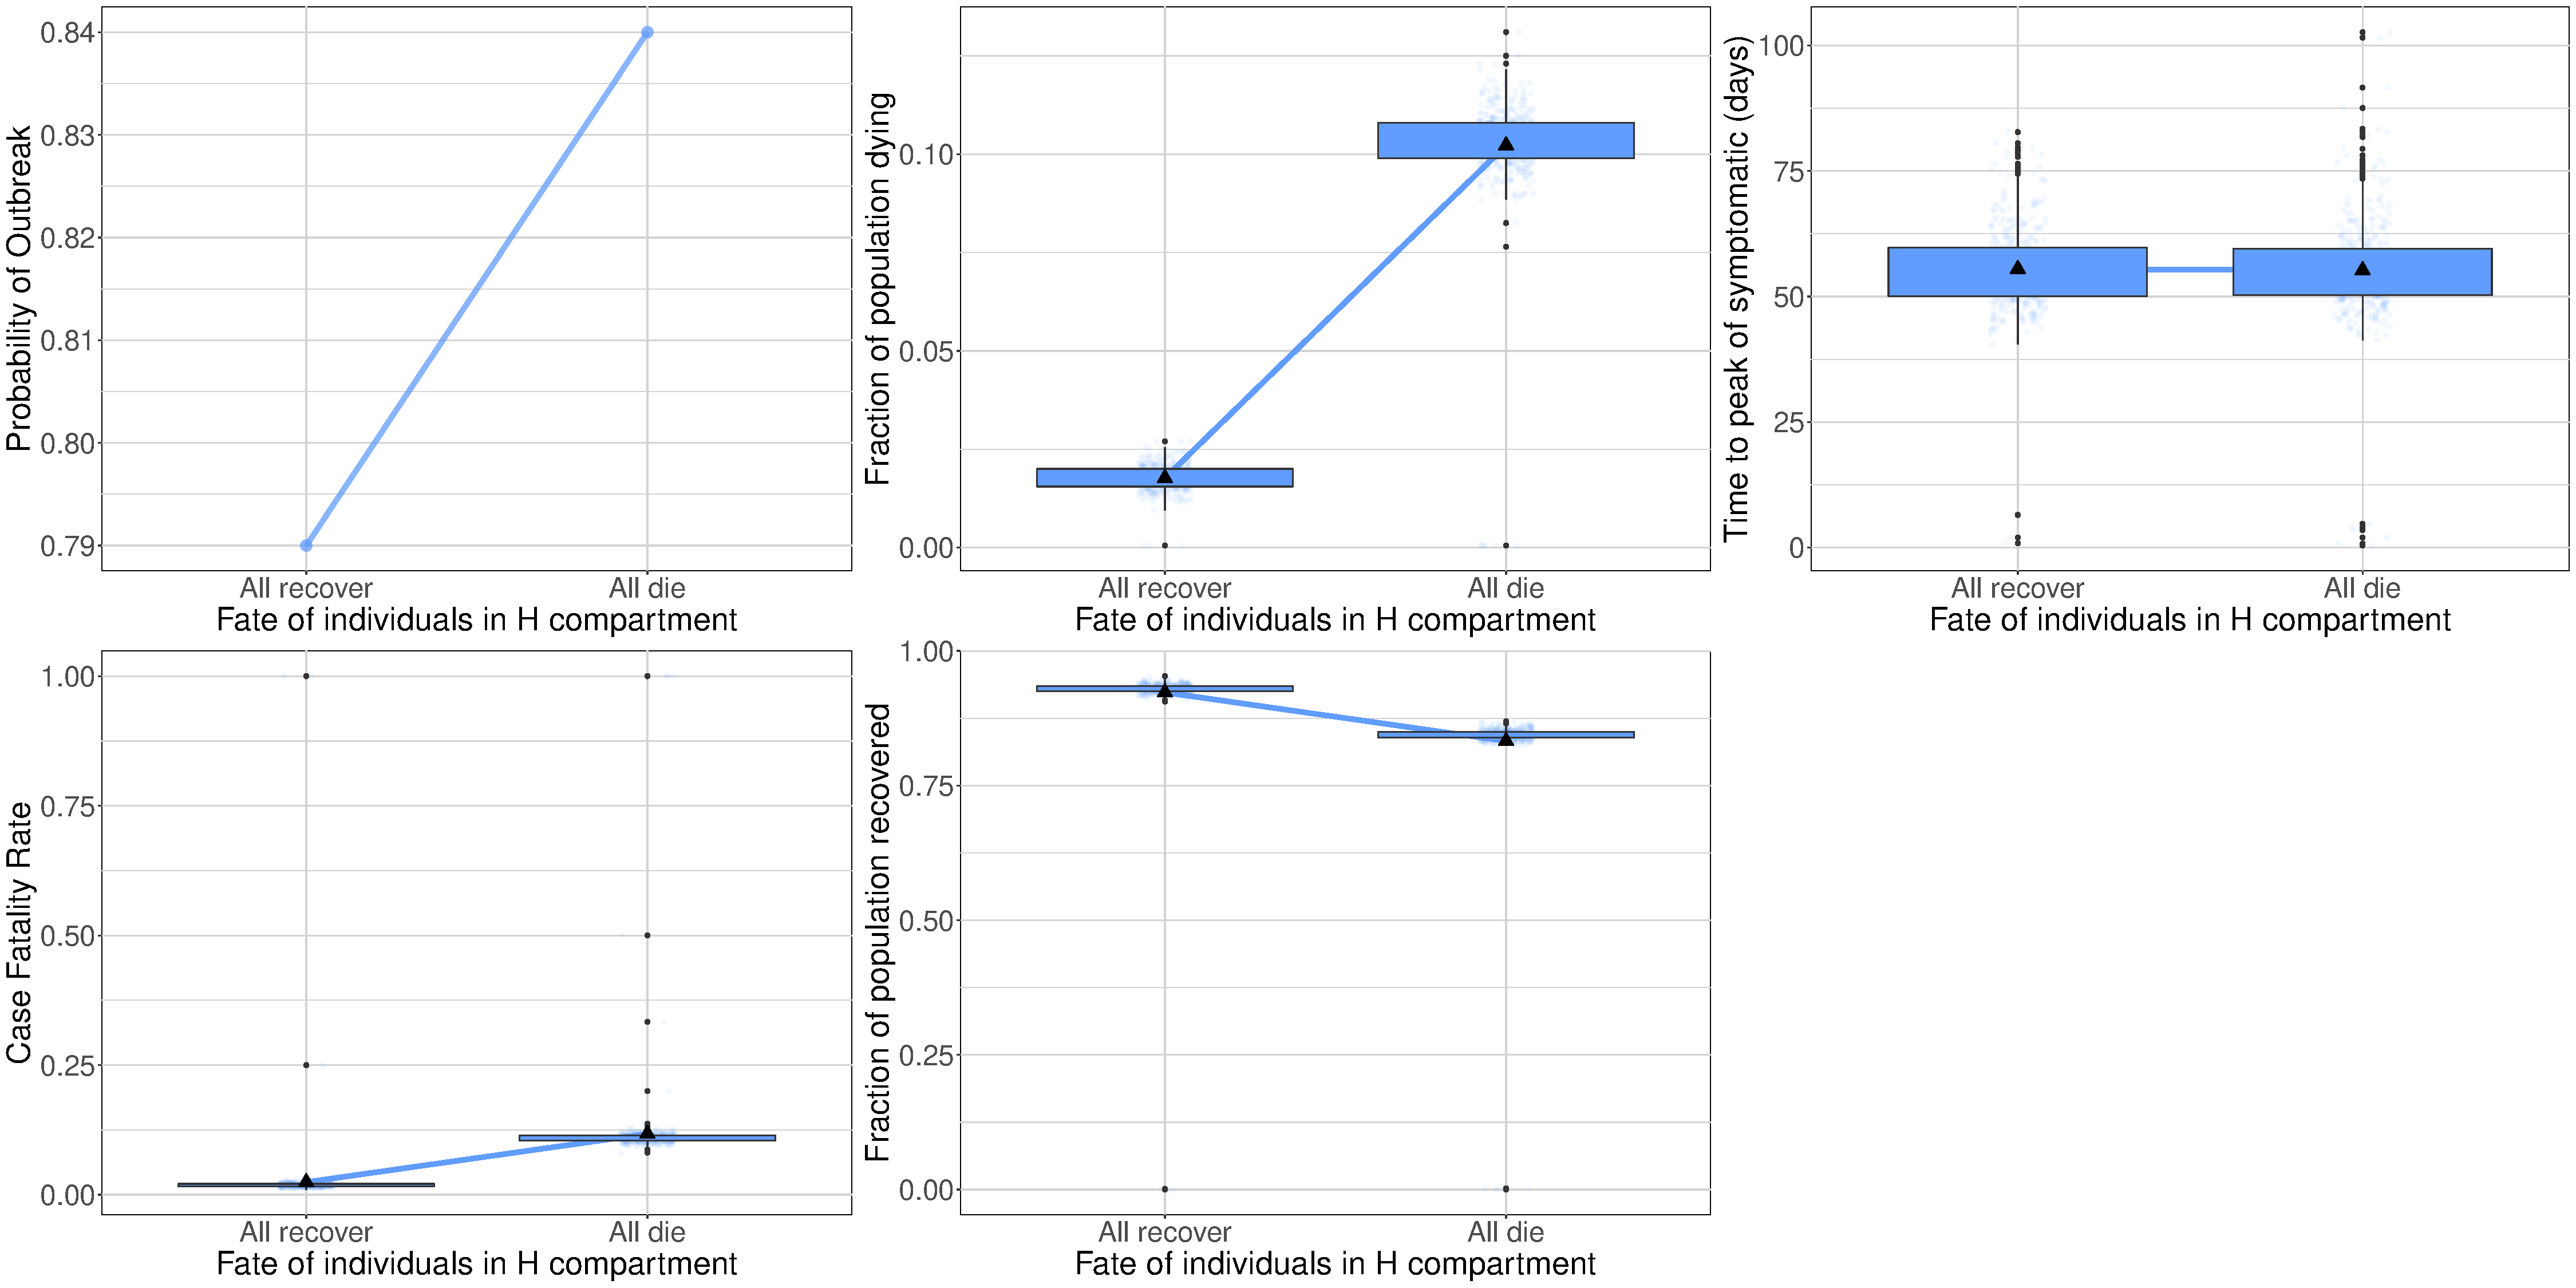
\includegraphics[width=1\textwidth]{figures/FigS2}\hspace{2mm}\caption{\label{fig:Suppl_DvsR} \textbf{Outcomes when all severe (hospitalized)
cases recover ($\sigma=0$) vs when all severe (hospitalized) cases
die ($\sigma=1$).} Probability of an outbreak (top left), fraction
of the population dying (top middle), time until peak symptomatic
cases (top right), IFR (bottom left), and fraction of the population
that recovers (bottom middle). Since we define outbreaks as simulations
in which at least one person dies and probability of a case dying
is higher when $\sigma=1$, the probability of observing an outbreak
is also necessarily higher when$\sigma=1.$}
\end{figure}

\medskip{}

\begin{figure}[H]
\centering{}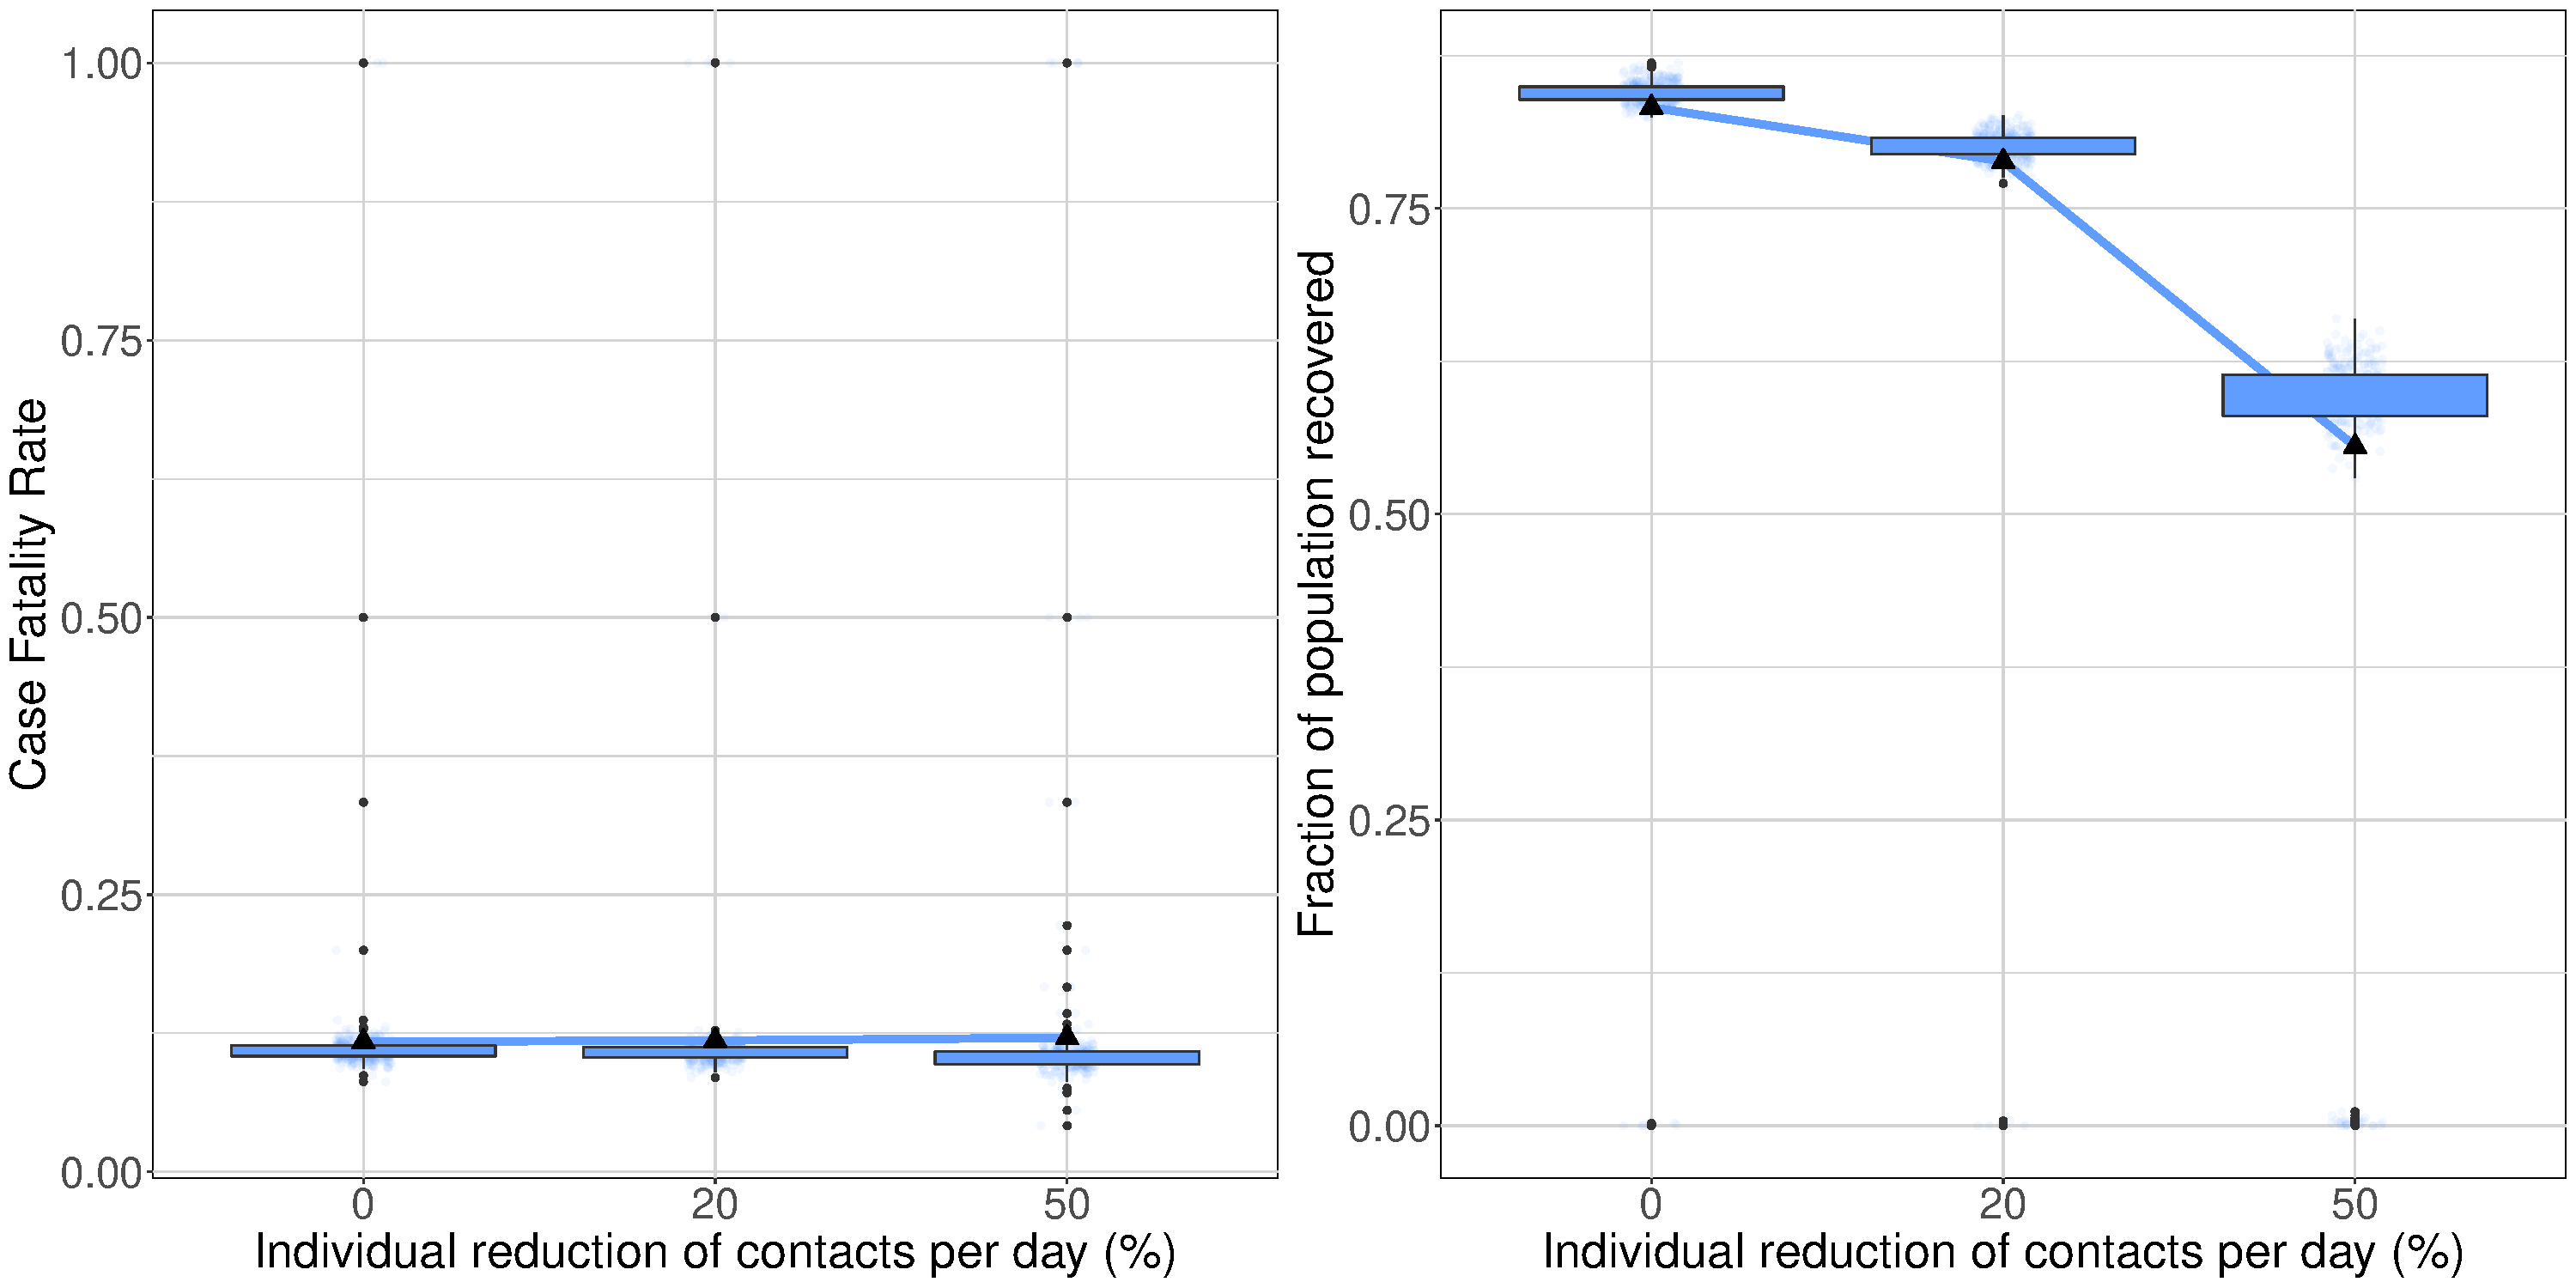
\includegraphics[width=1\textwidth]{figures/FigS3}\hspace{2mm}\caption{\label{fig:Suppl_self} \textbf{Self-distancing.} IFR (left), and
fraction of the population that recovers (right) as a function of
the proportion of contacts reduced per individual per day.}
\end{figure}
\medskip{}

\begin{figure}[H]
\centering{}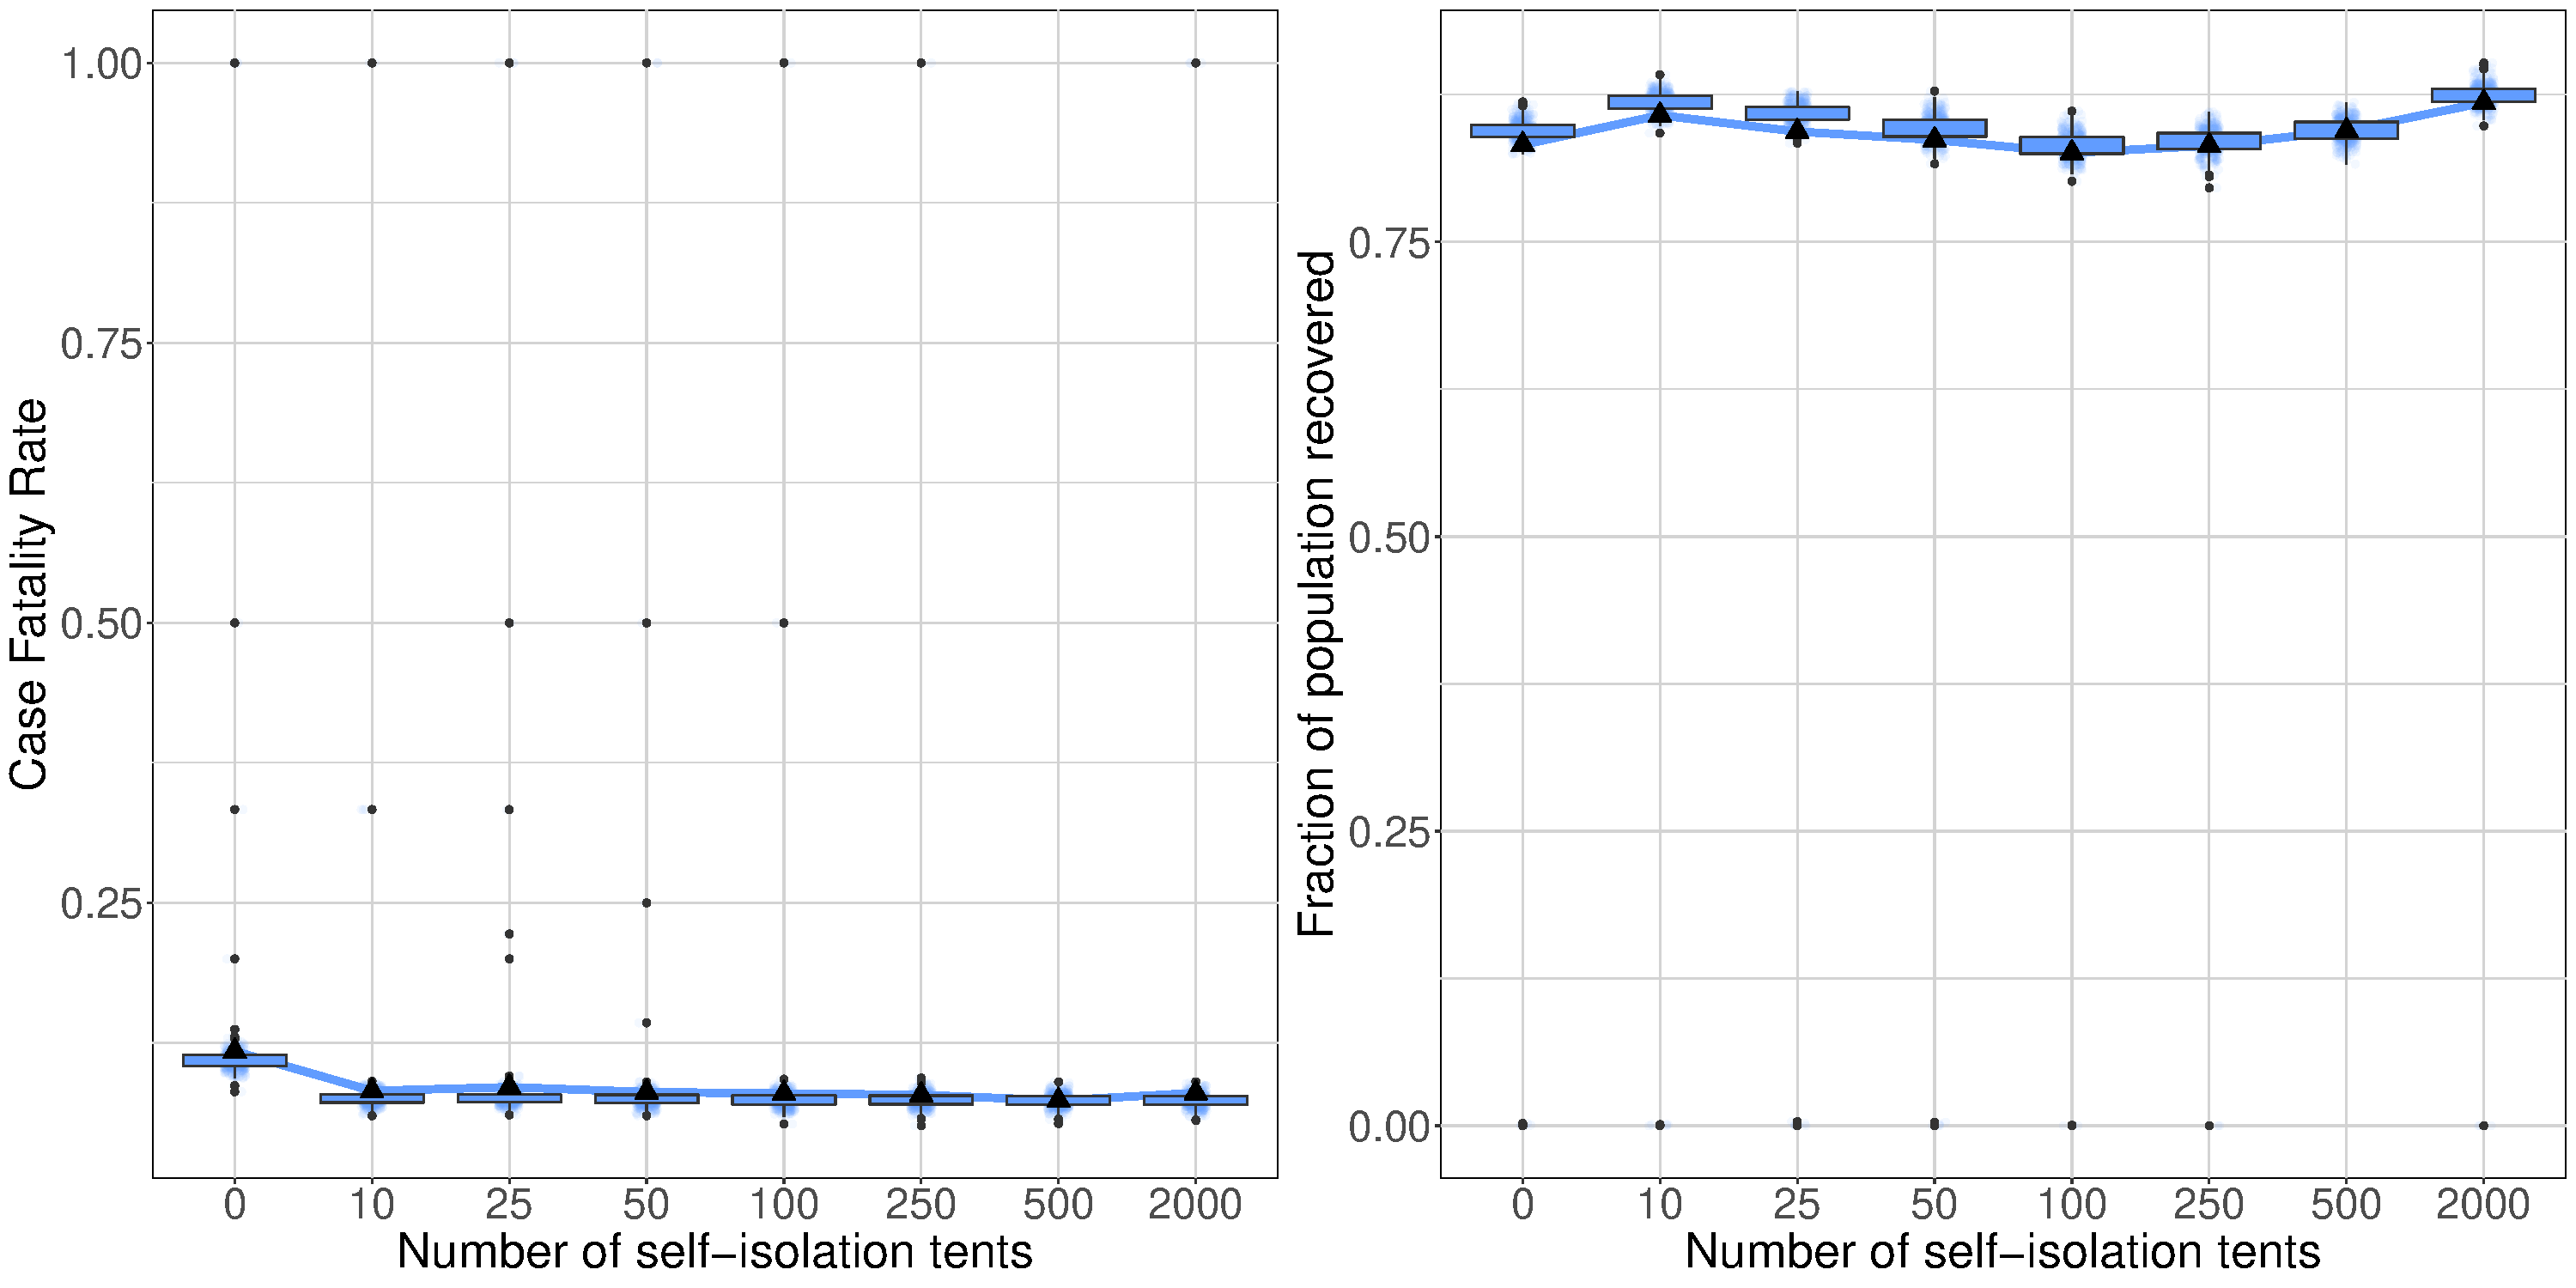
\includegraphics[width=1\textwidth]{figures/FigS4}\hspace{2mm}\caption{\label{fig:Suppl_isolation} \textbf{Self-isolation.} IFR (left),
and fraction of the population that recovers (right) as a function
of the number of isolation tents available in the camp.}
\end{figure}

\medskip{}

\begin{figure}[H]
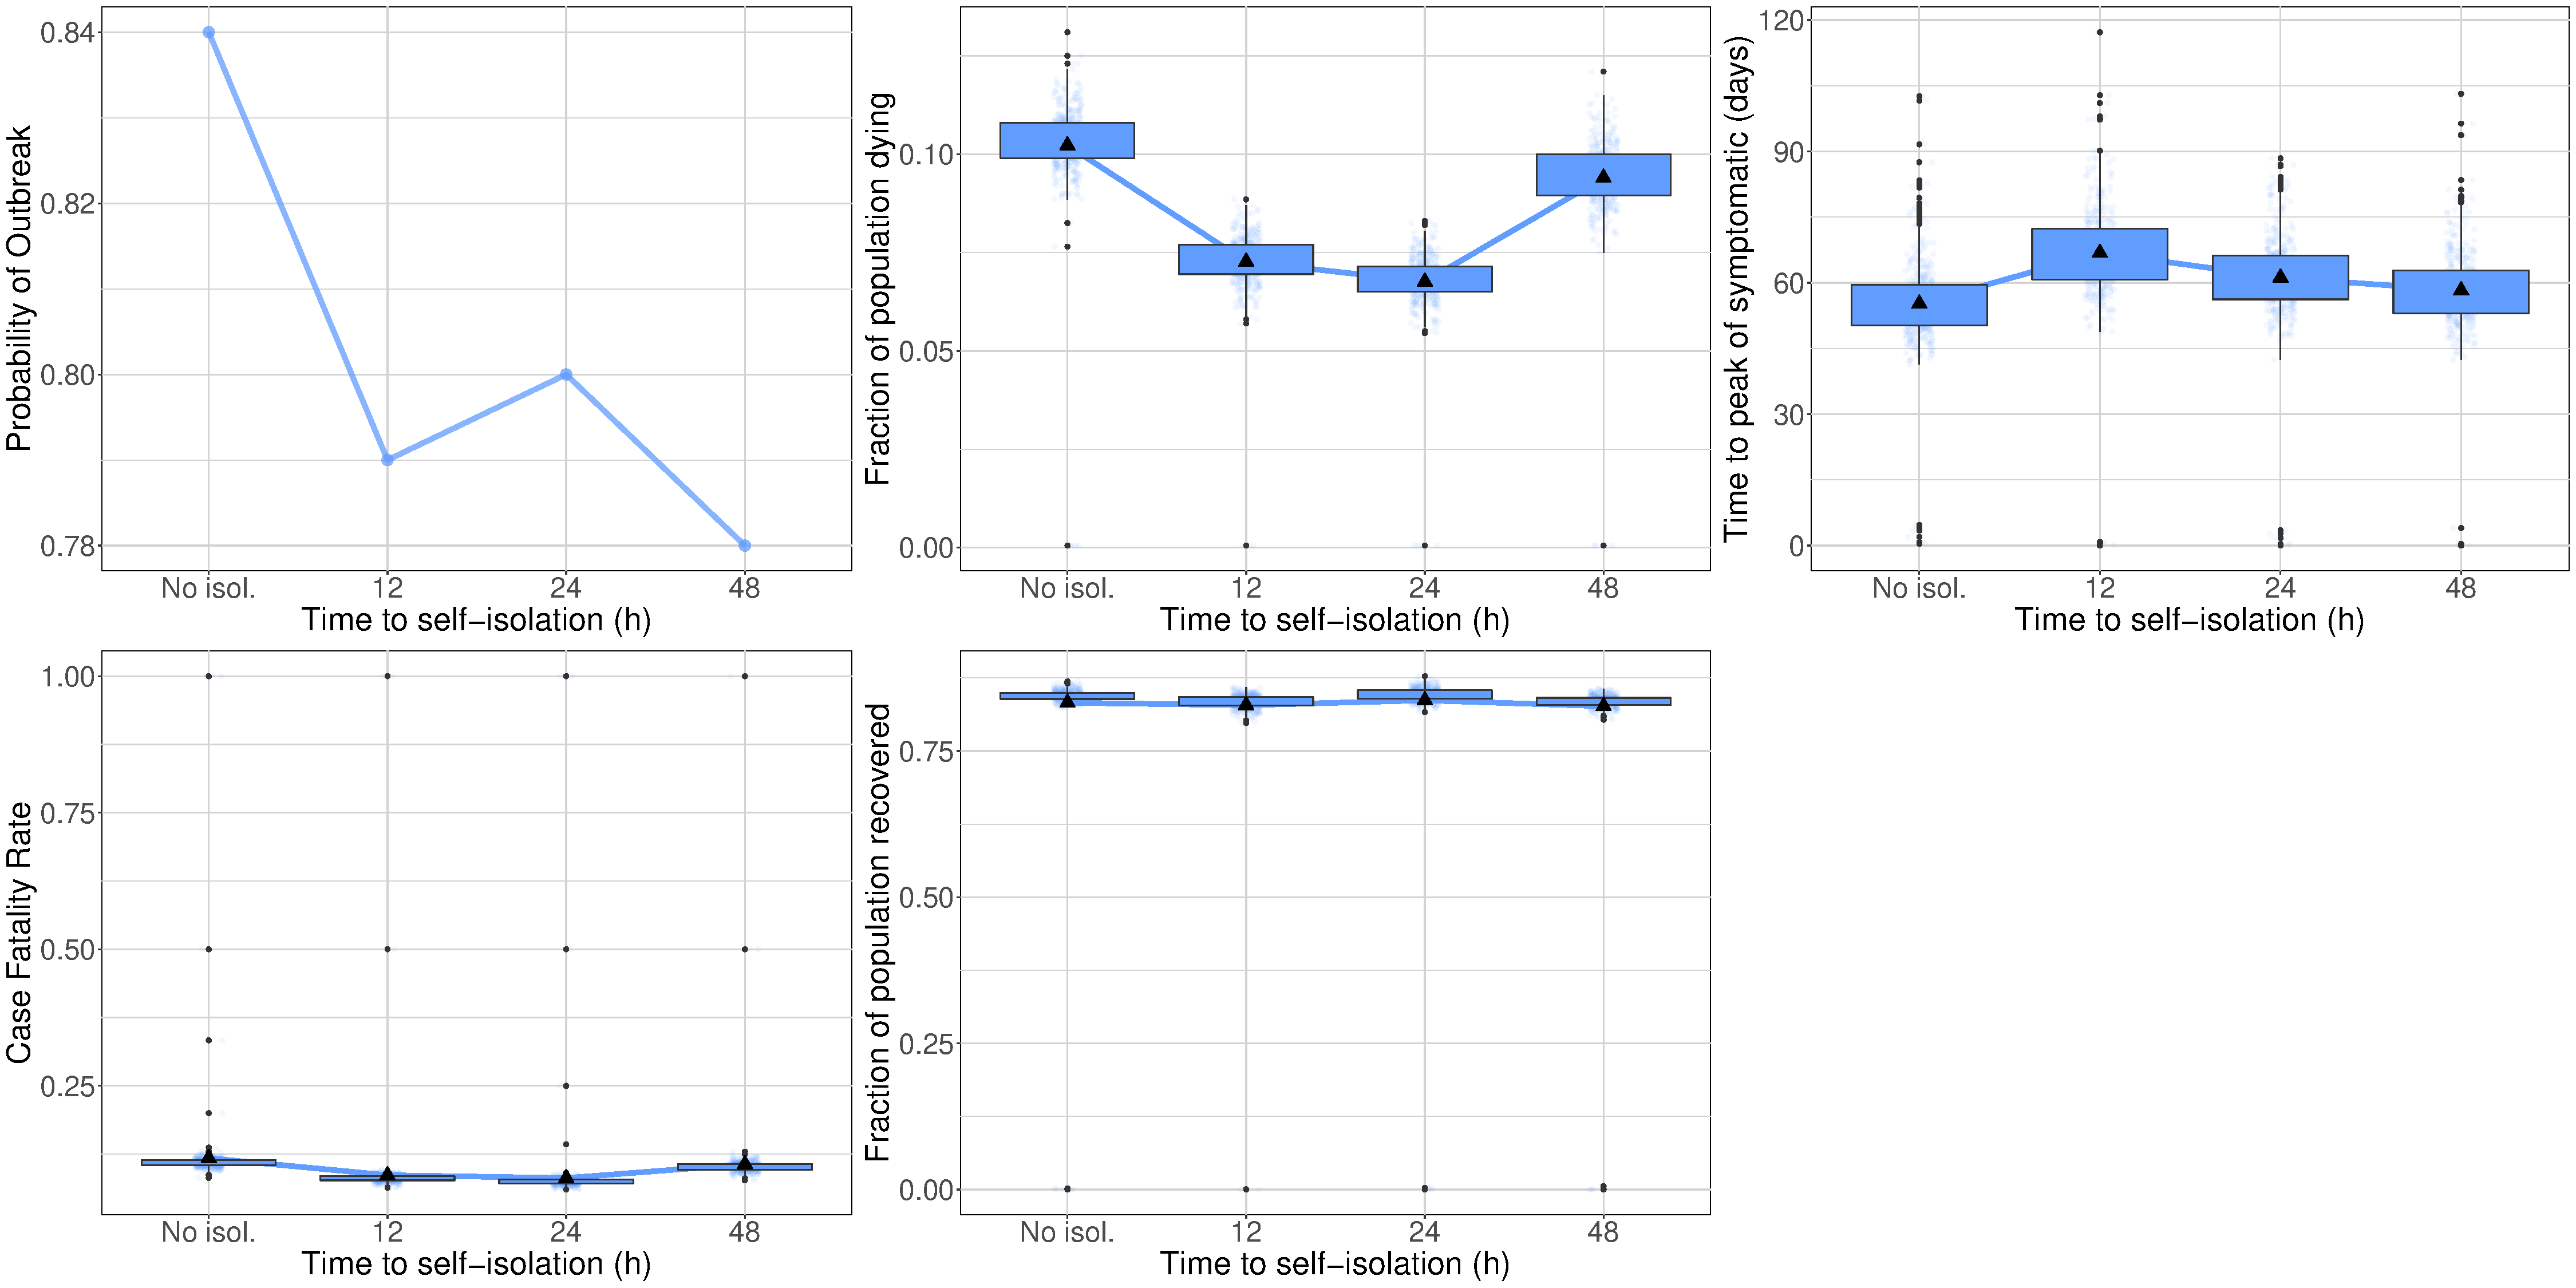
\includegraphics[width=1\textwidth]{figures/FigS5}\hspace{2mm}\caption{\label{fig:Suppl_onset} \textbf{Time to self-isolation.} Probability
of an outbreak (top left), fraction of the population dying (top middle),
time until peak symptomatic cases (top right), IFR (bottom left),
and fraction of the population that recovers (bottom middle) as a
function of the time that individuals require to recognize their symptoms
and self-isolate.}
\end{figure}

\medskip{}

\begin{figure}[H]
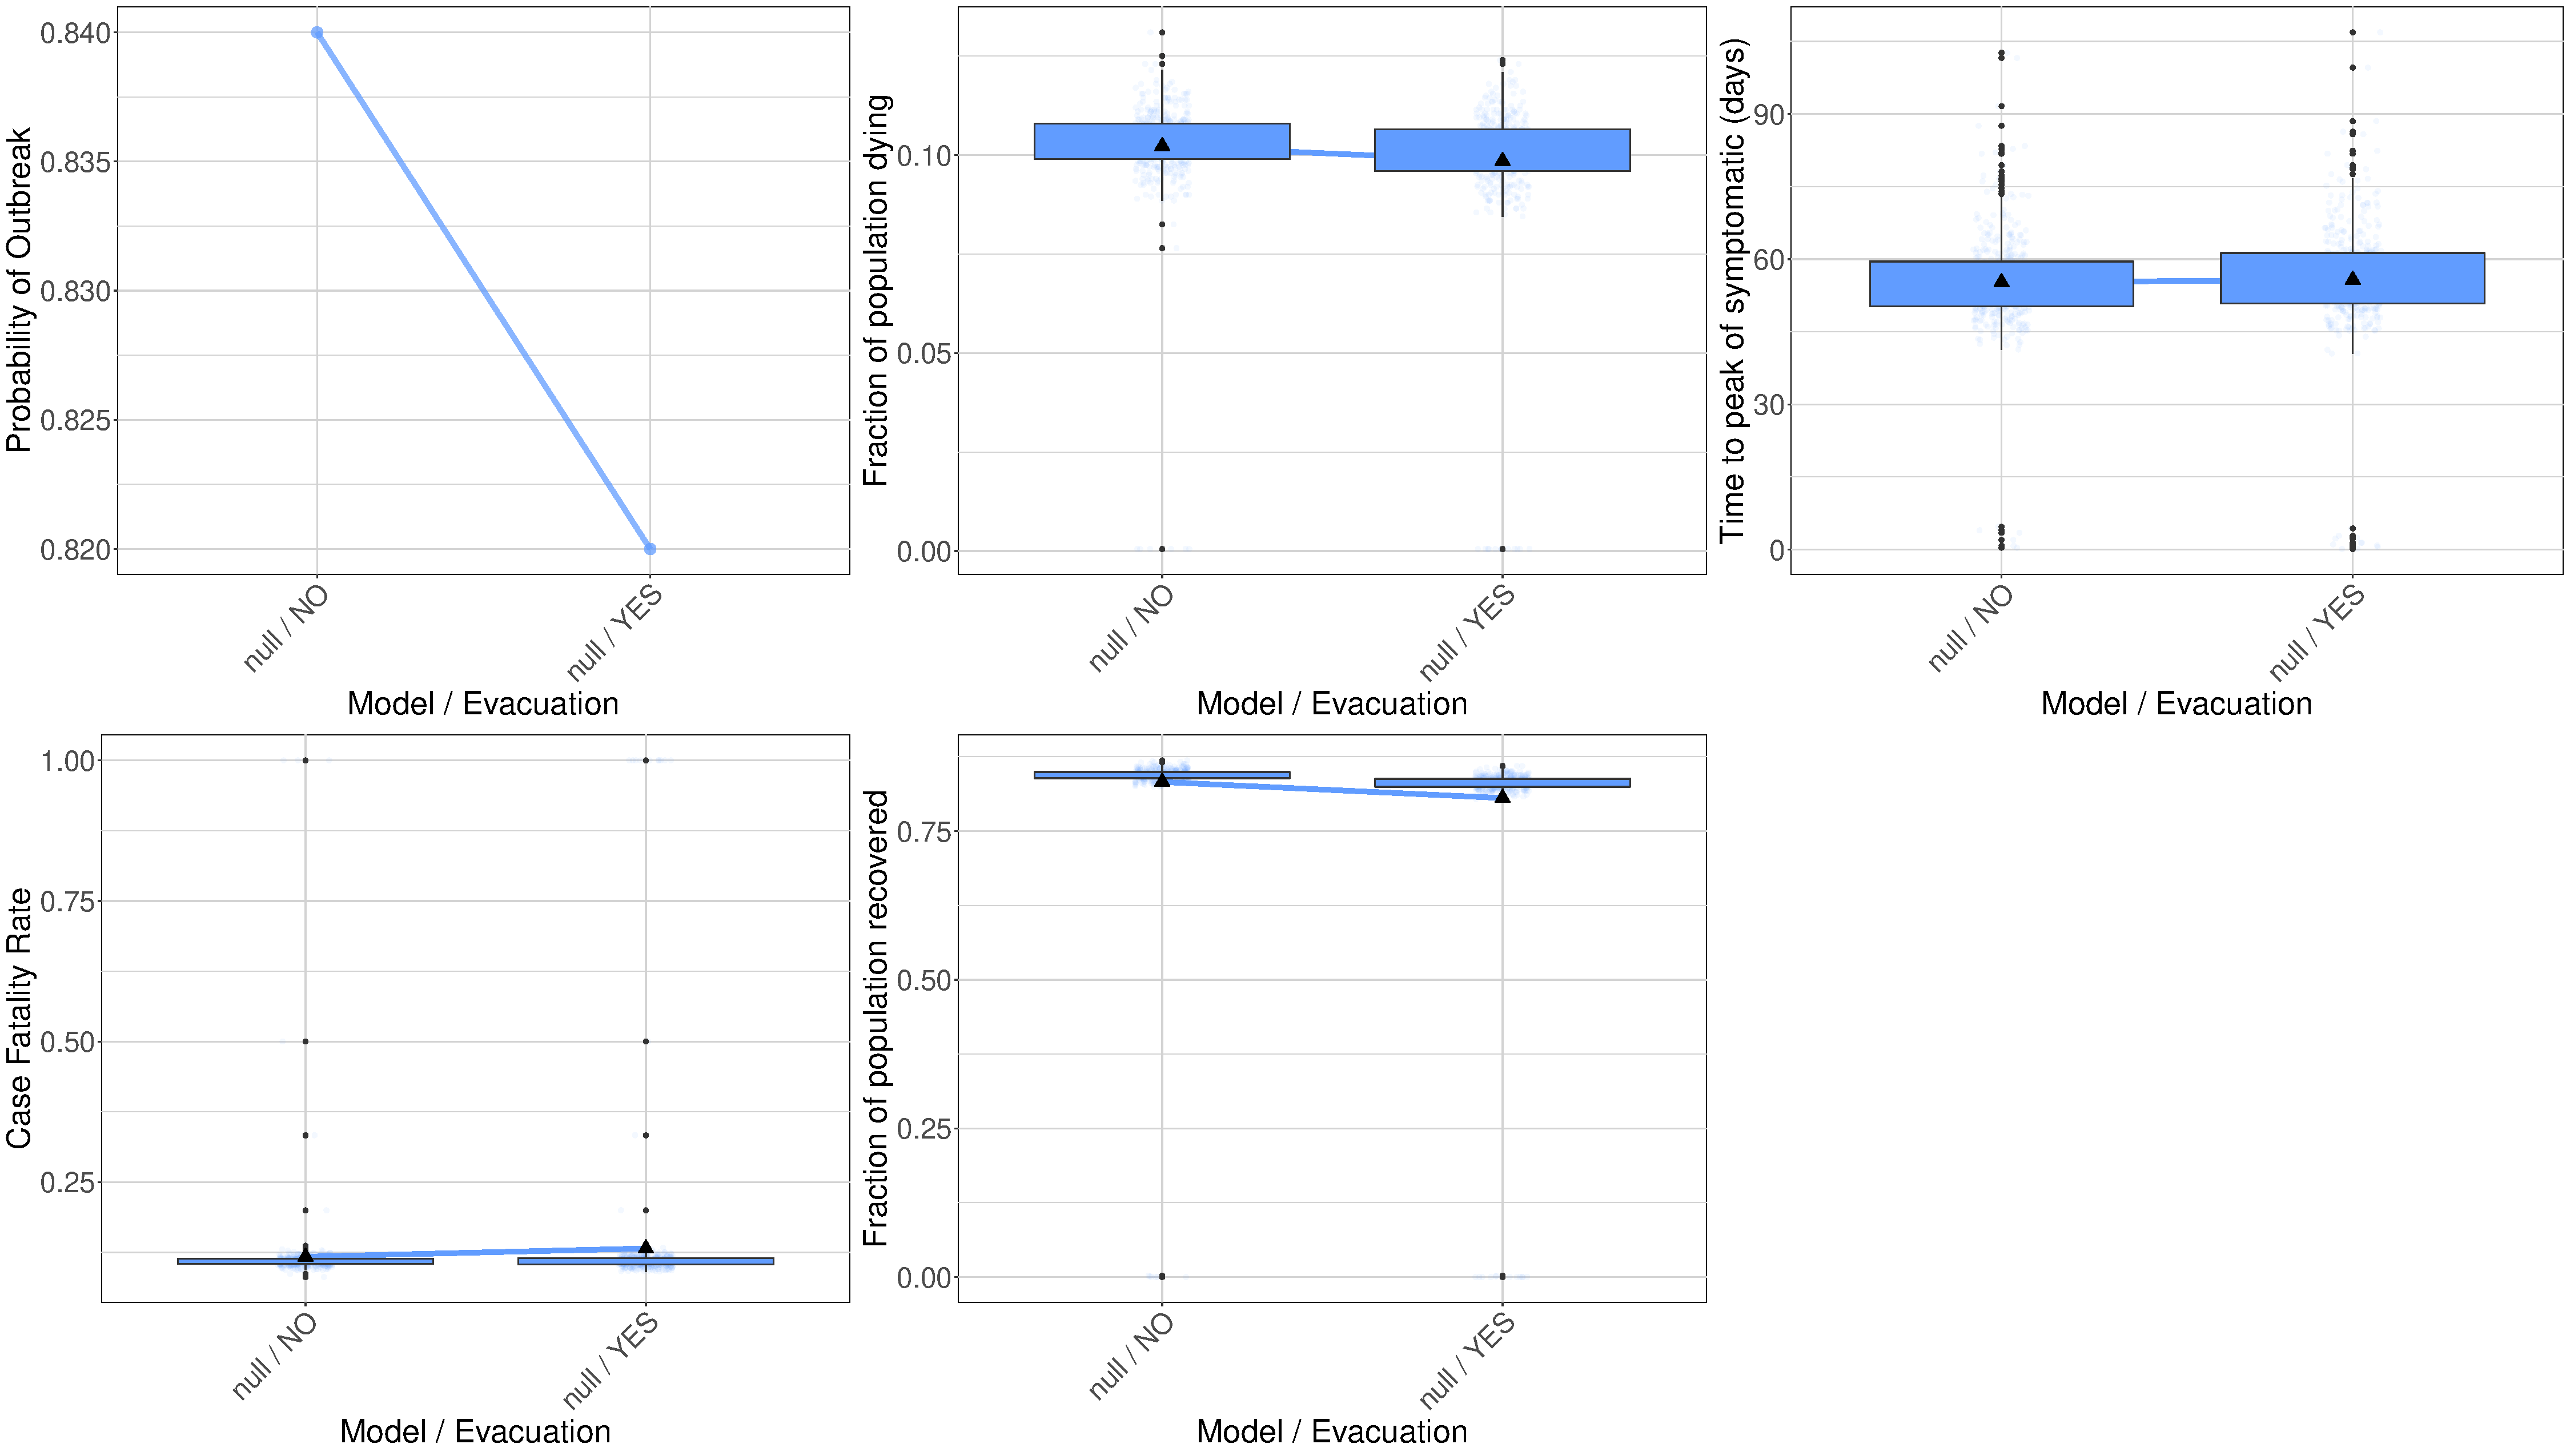
\includegraphics[width=1\textwidth]{figures/FigS6}\hspace{2mm}\caption{\label{fig:Suppl_evacuation} \textbf{Evacuation.} Probability of
an outbreak (top left), fraction of the population dying (top middle),
time until peak symptomatic cases (top right), IFR (bottom left),
and fraction of the population that recovers (bottom middle), as a
function of whether individuals requiring hospitalization are evacuated
to isolation centers.}
\end{figure}

\medskip{}

\begin{figure}[H]
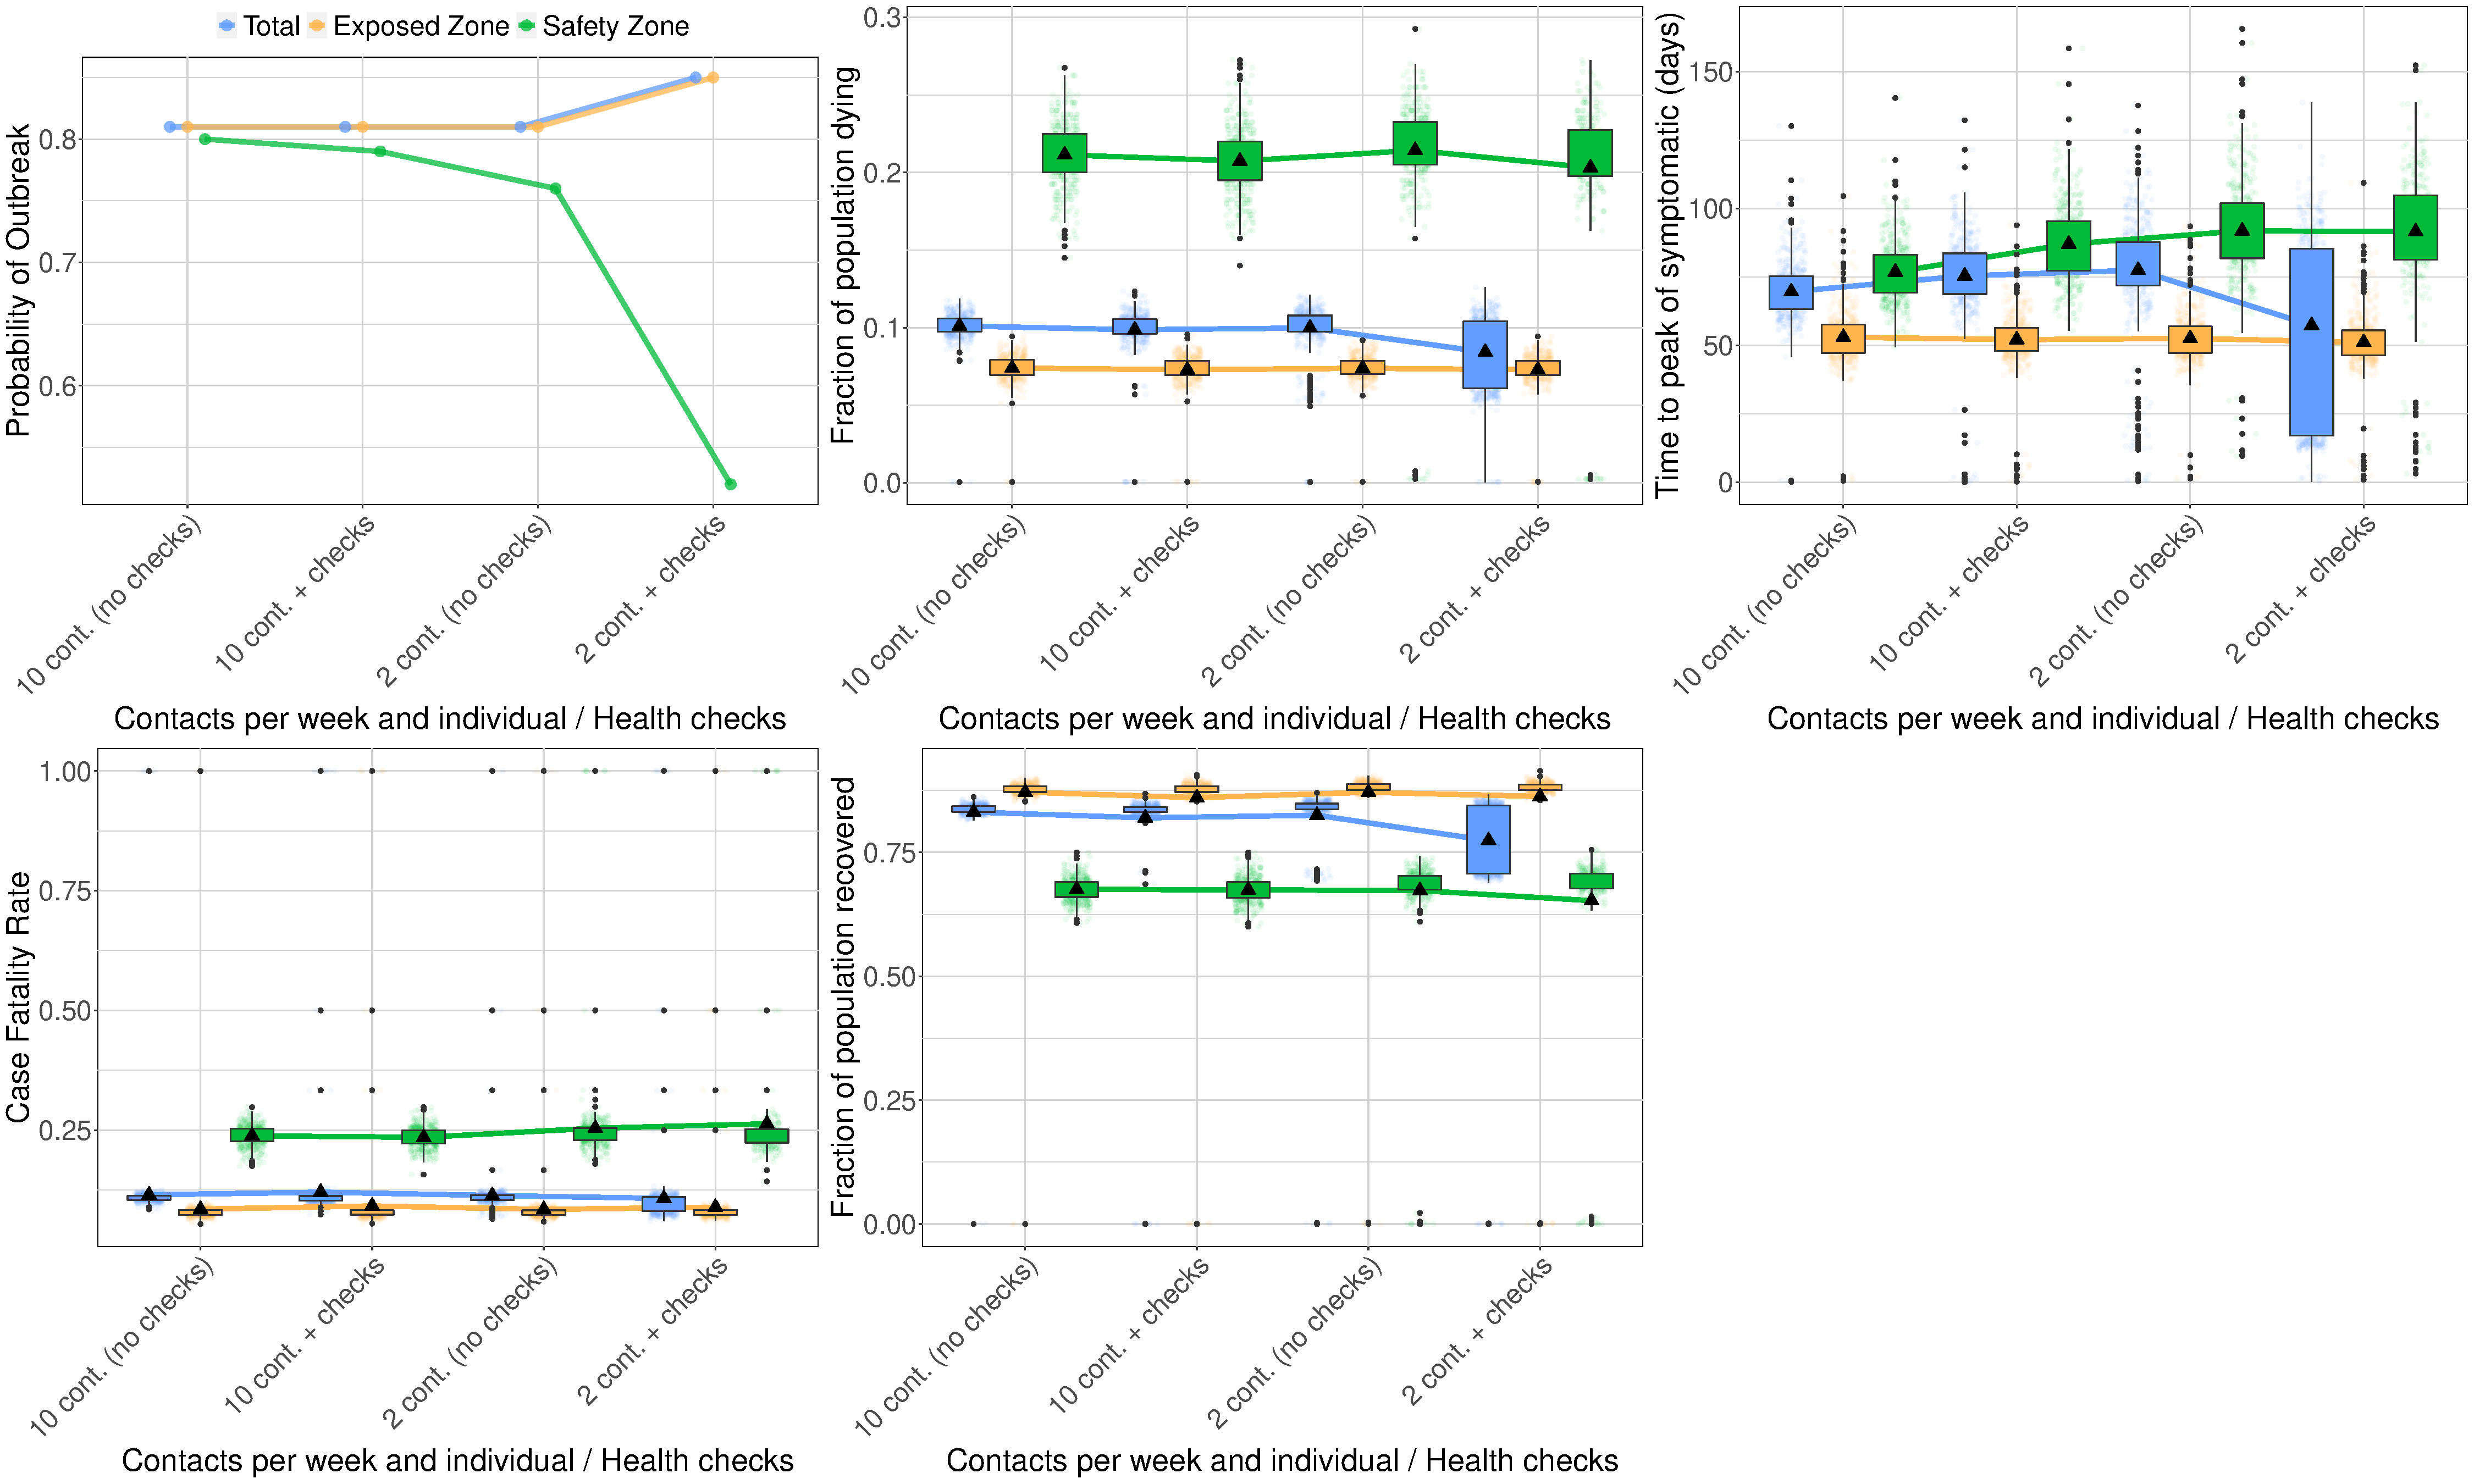
\includegraphics[width=1\textwidth]{figures/FigS7}\hspace{2mm}\caption{\label{fig:Suppl_Tcheck} \textbf{Health-checks in the buffer zone.}
Probability of an outbreak (top left), fraction of the population
dying (top middle), time until peak symptomatic cases (top right),
IFR (bottom left), and fraction of the population that recovers (bottom
middle), as a function of whether health-checks are implemented in
the buffer zone between the safety and exposed zones. Scenarios with
10 or 2 contacts in the buffer zone per person in the safety zone
per week are plotted. All figures consider the scenario in which 20\%
of the camp's population is allocated to the safety zone.}
\end{figure}

\begin{figure}[H]
\centering{}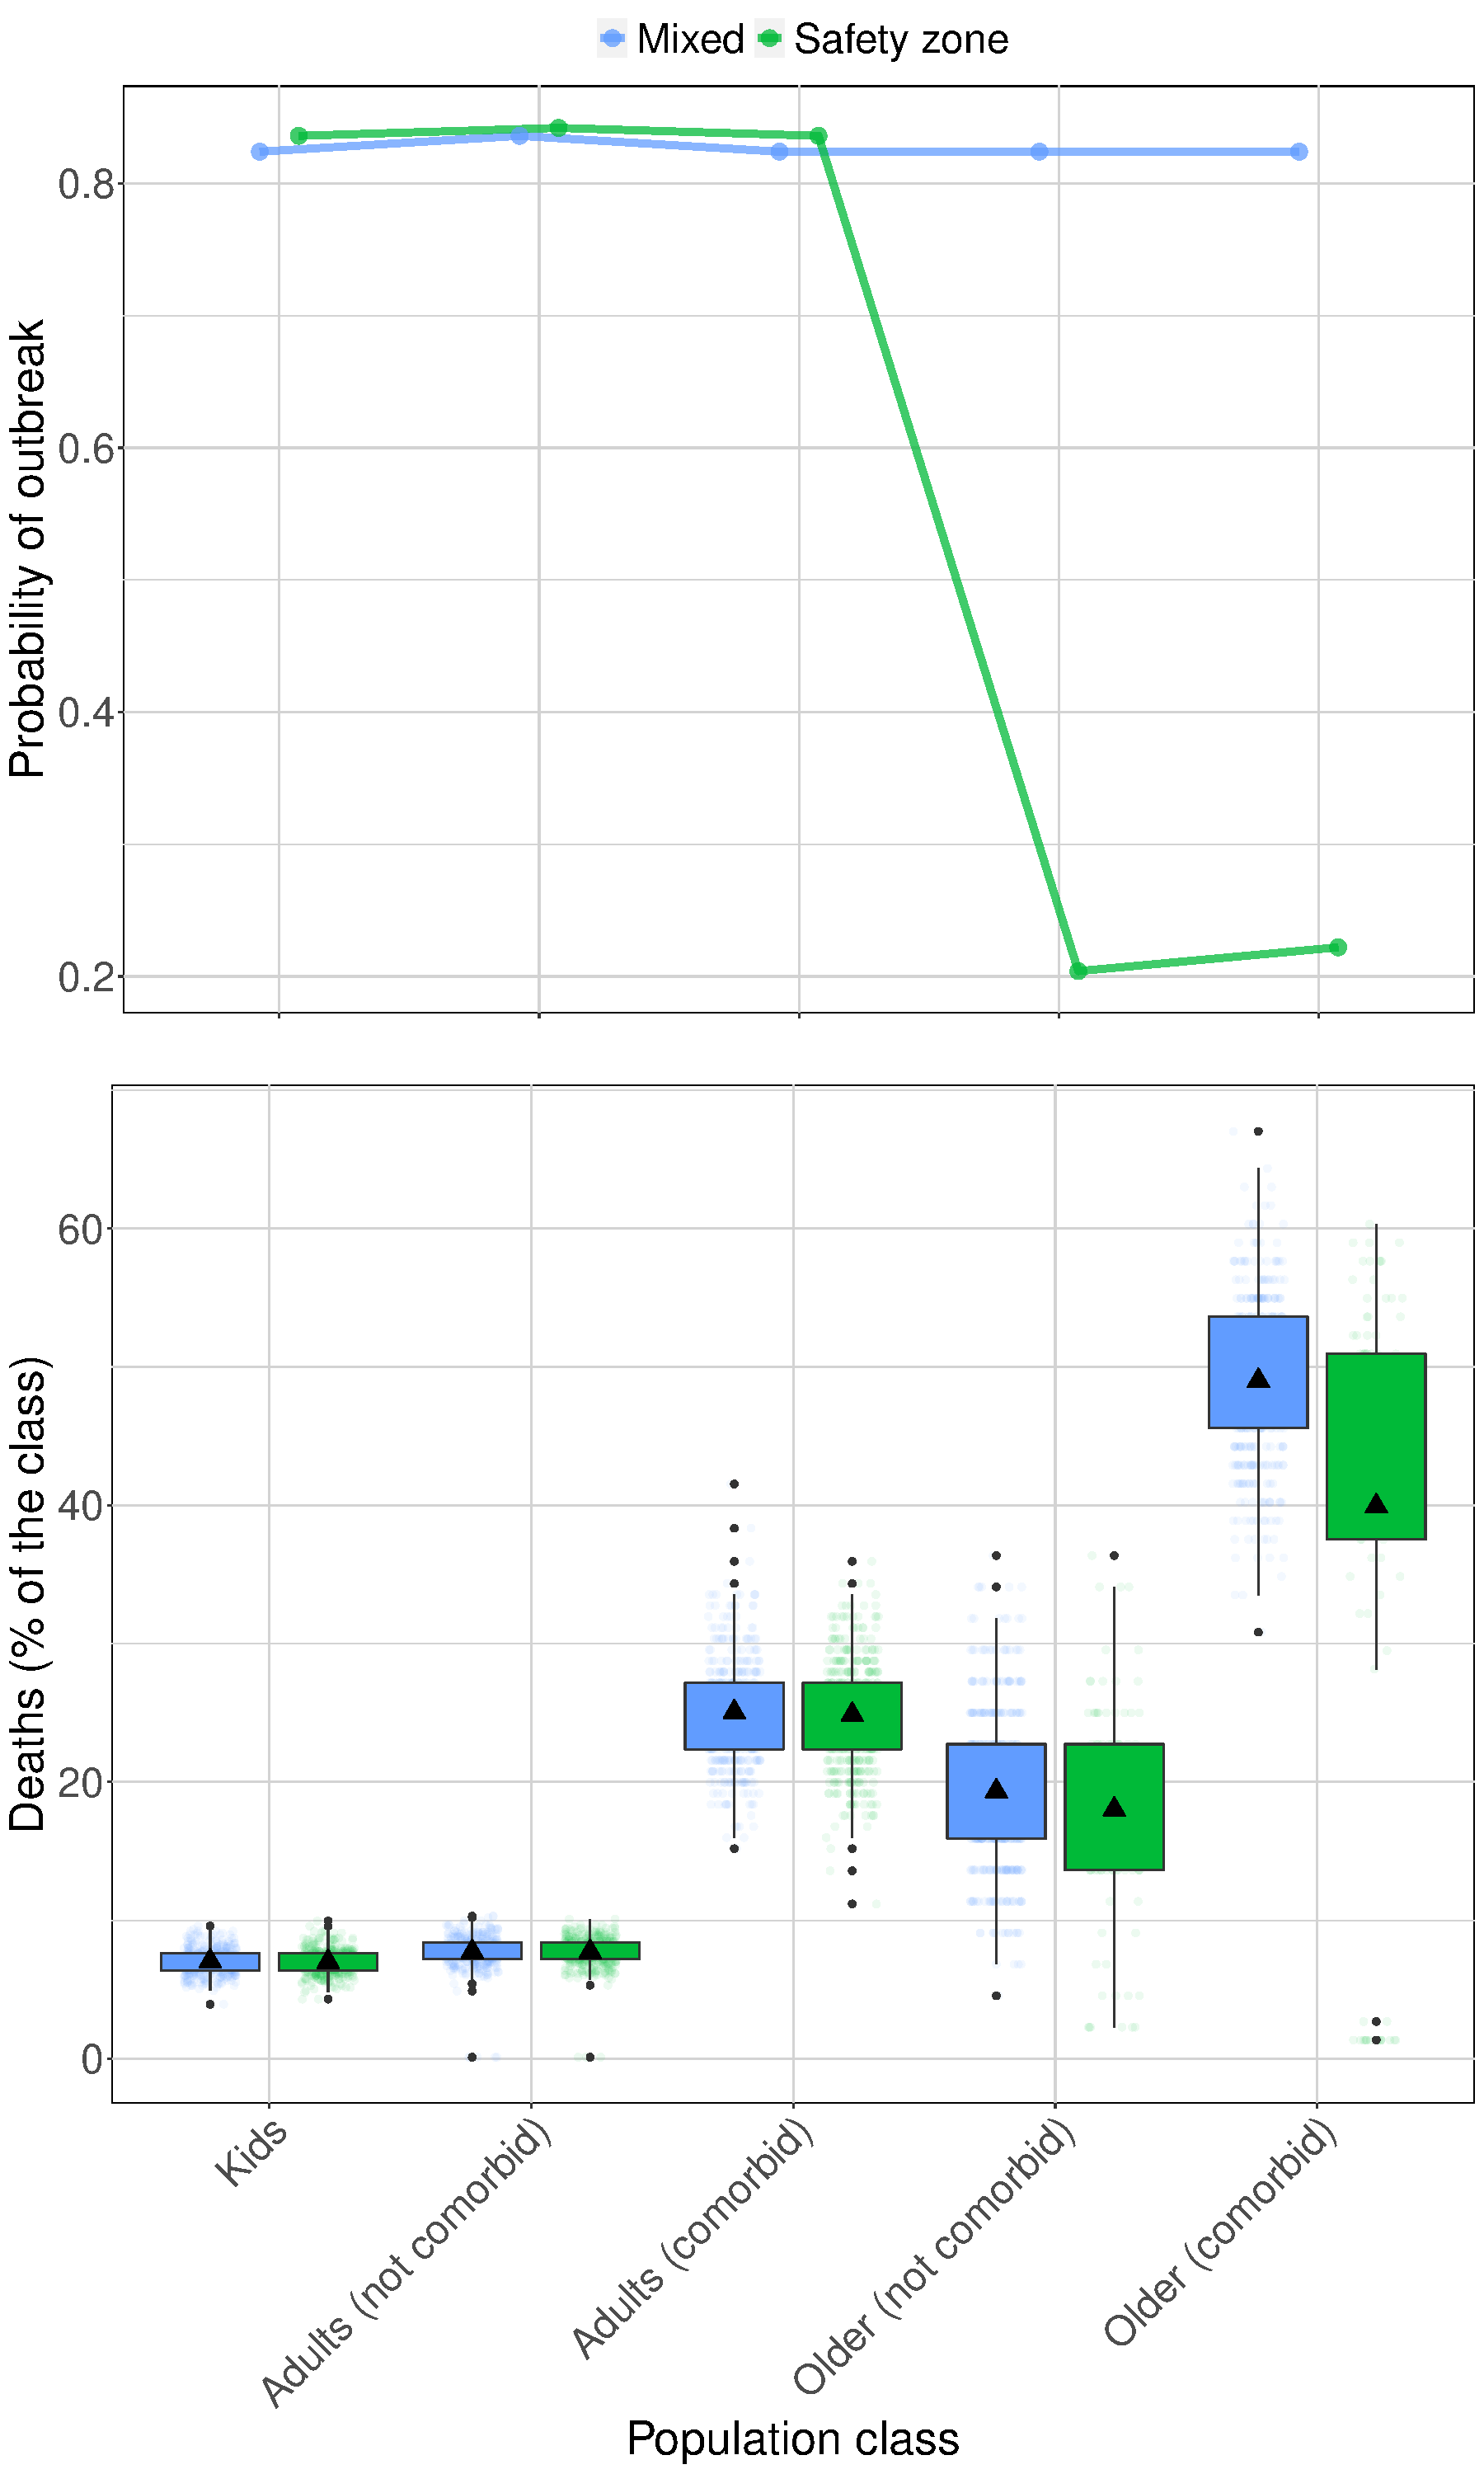
\includegraphics[width=0.6\textwidth]{figures/FigS8}\hspace{2mm}\caption{\label{fig:Suppl_agegroups} \textbf{Effects of the safety zone on
outcomes by population class. }Probability of an outbreak (top), and
proportion that dies in each population class (bottom) when no interventions
are implemented (Mixed), compared to protection of older adults in
the safety zone with 2 contacts in the buffer zone per week (Safety
zone). The fraction of deaths in the safety zone for the older population
is significantly lower (Kruskal-Wallis test, p-val$<10^{-15}$).}
\end{figure}
\medskip{}

\begin{figure}[H]
\centering{}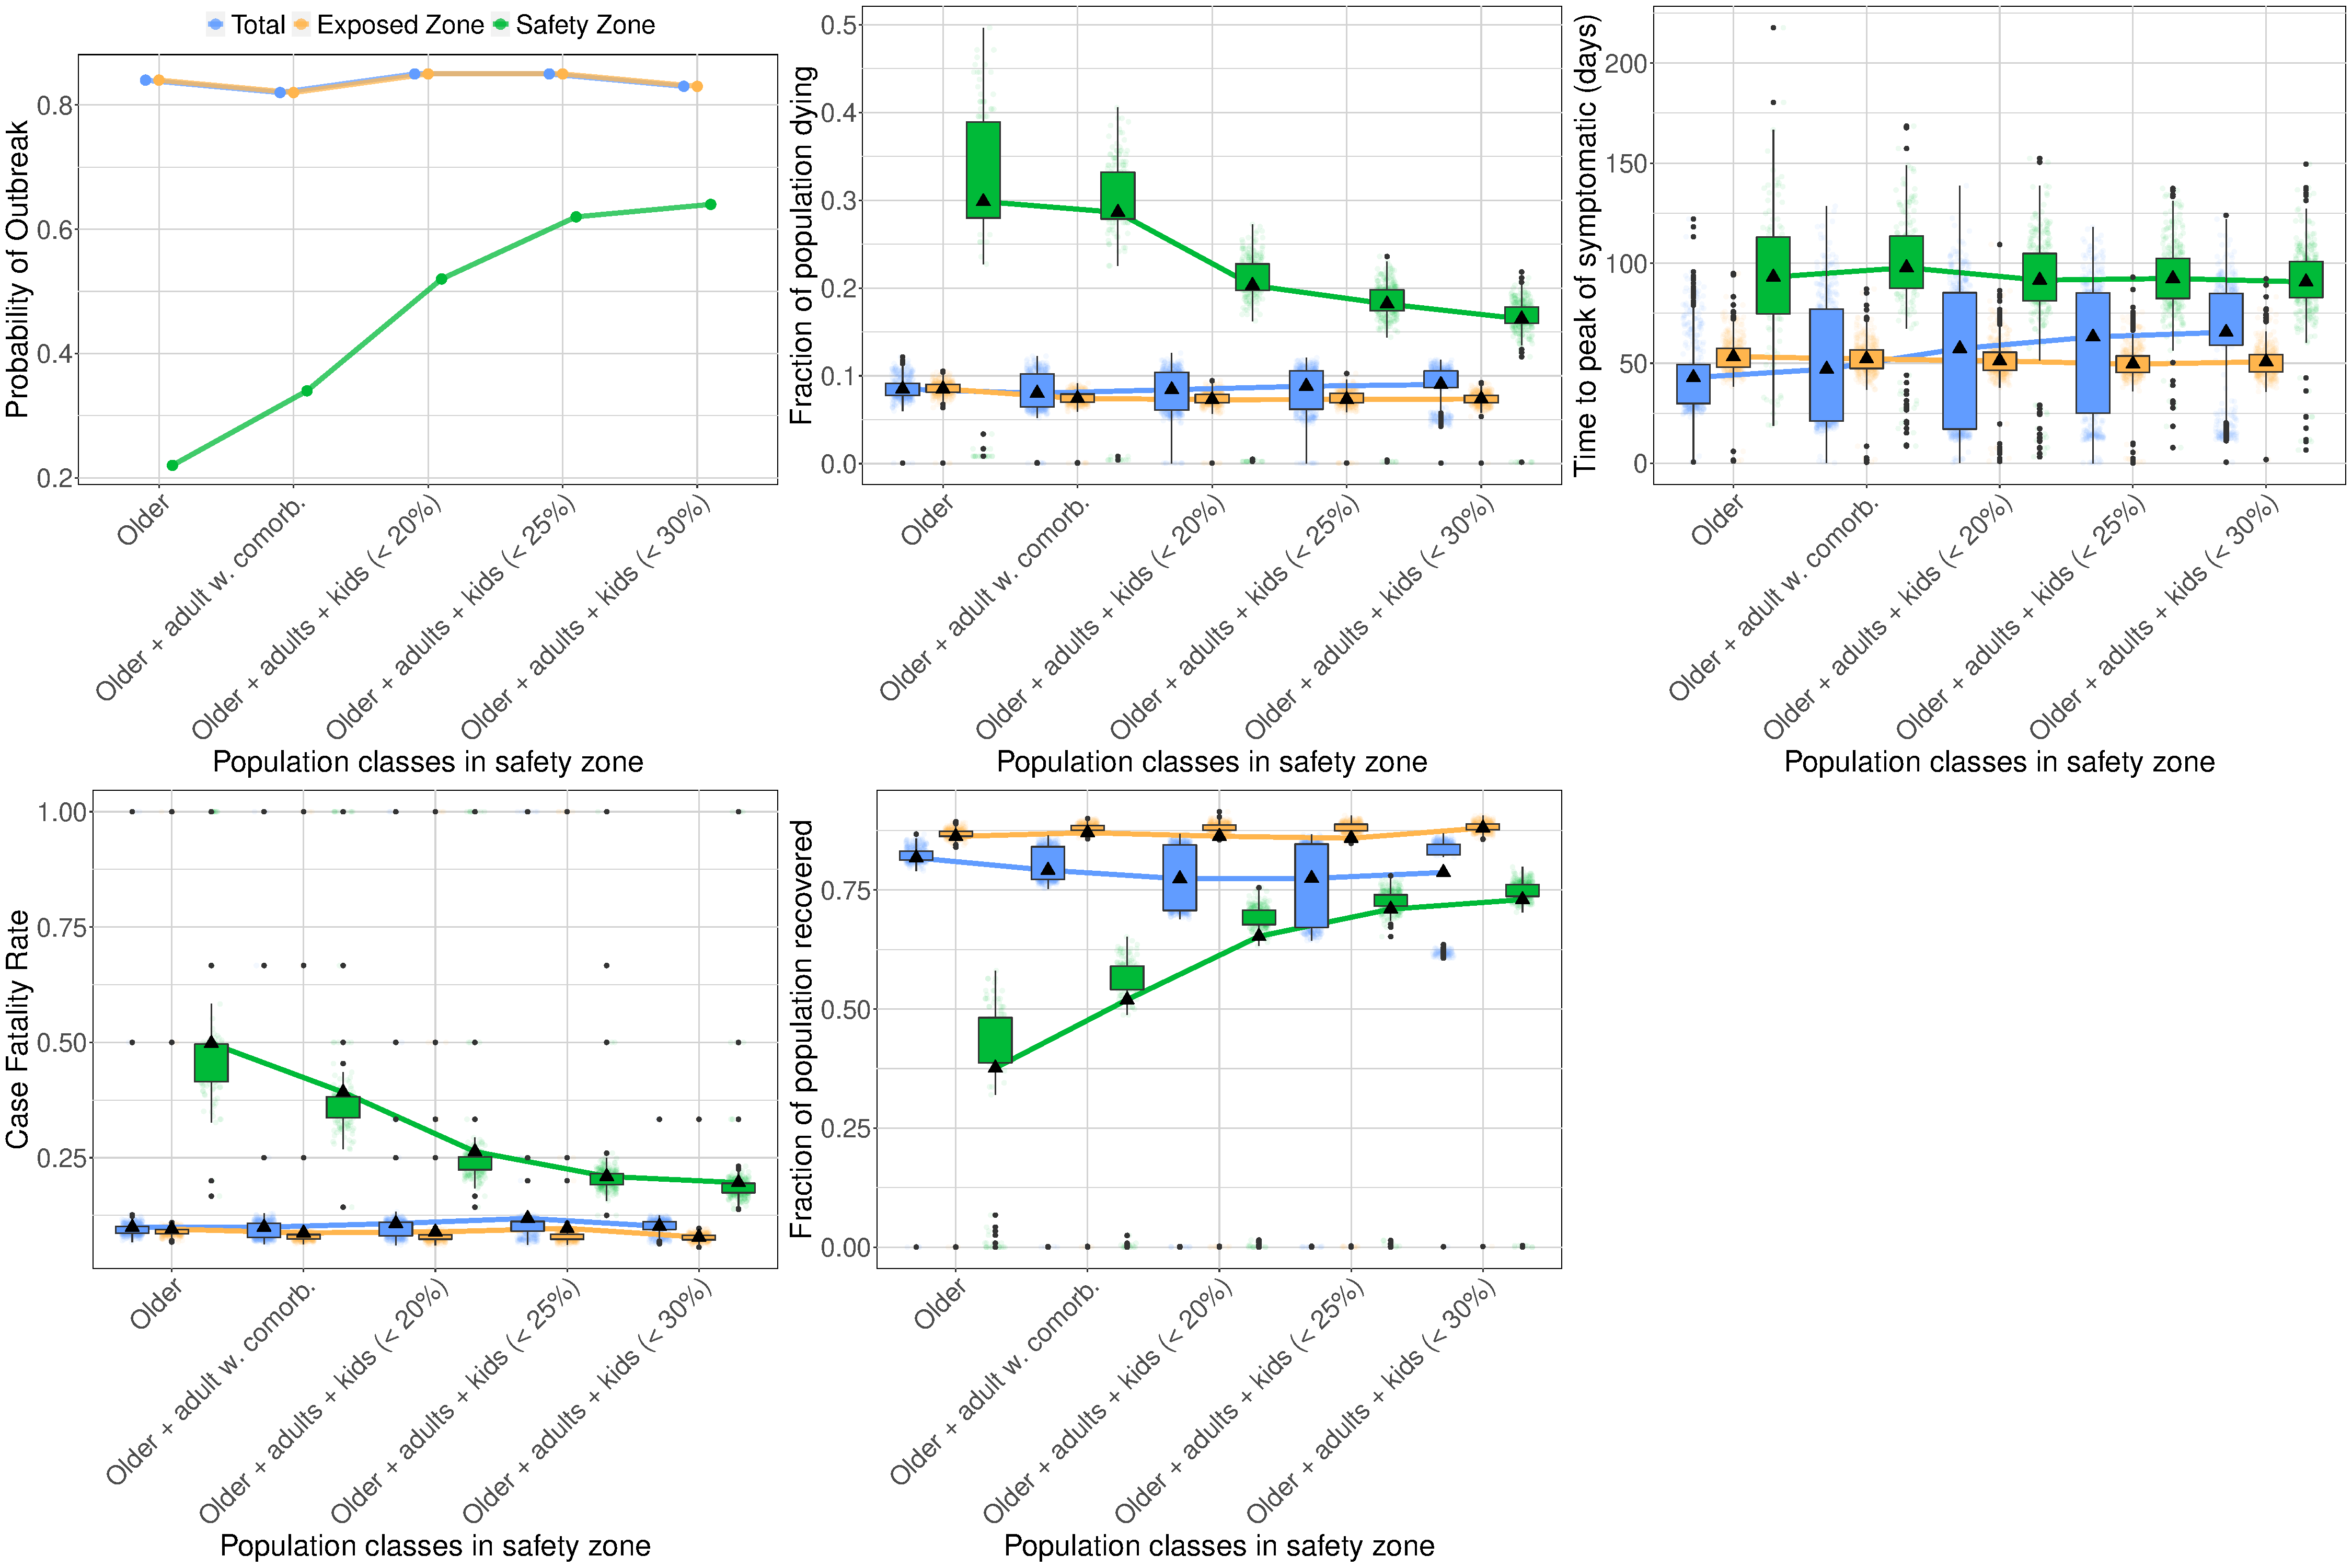
\includegraphics[width=1\textwidth]{figures/FigS9}\hspace{2mm}\caption{\label{fig:Suppl_safety} \textbf{Number of contacts in the buffer
zone.} IFR (left), and fraction of the population that recovers (right)
as a function of the number of contacts that each individual in the
safety zone has in the buffer zone per week. All figures consider
the scenario in which 20\% of the camp's population is allocated to
the safety zone.}
\end{figure}
\medskip{}

\begin{figure}[H]
\begin{centering}
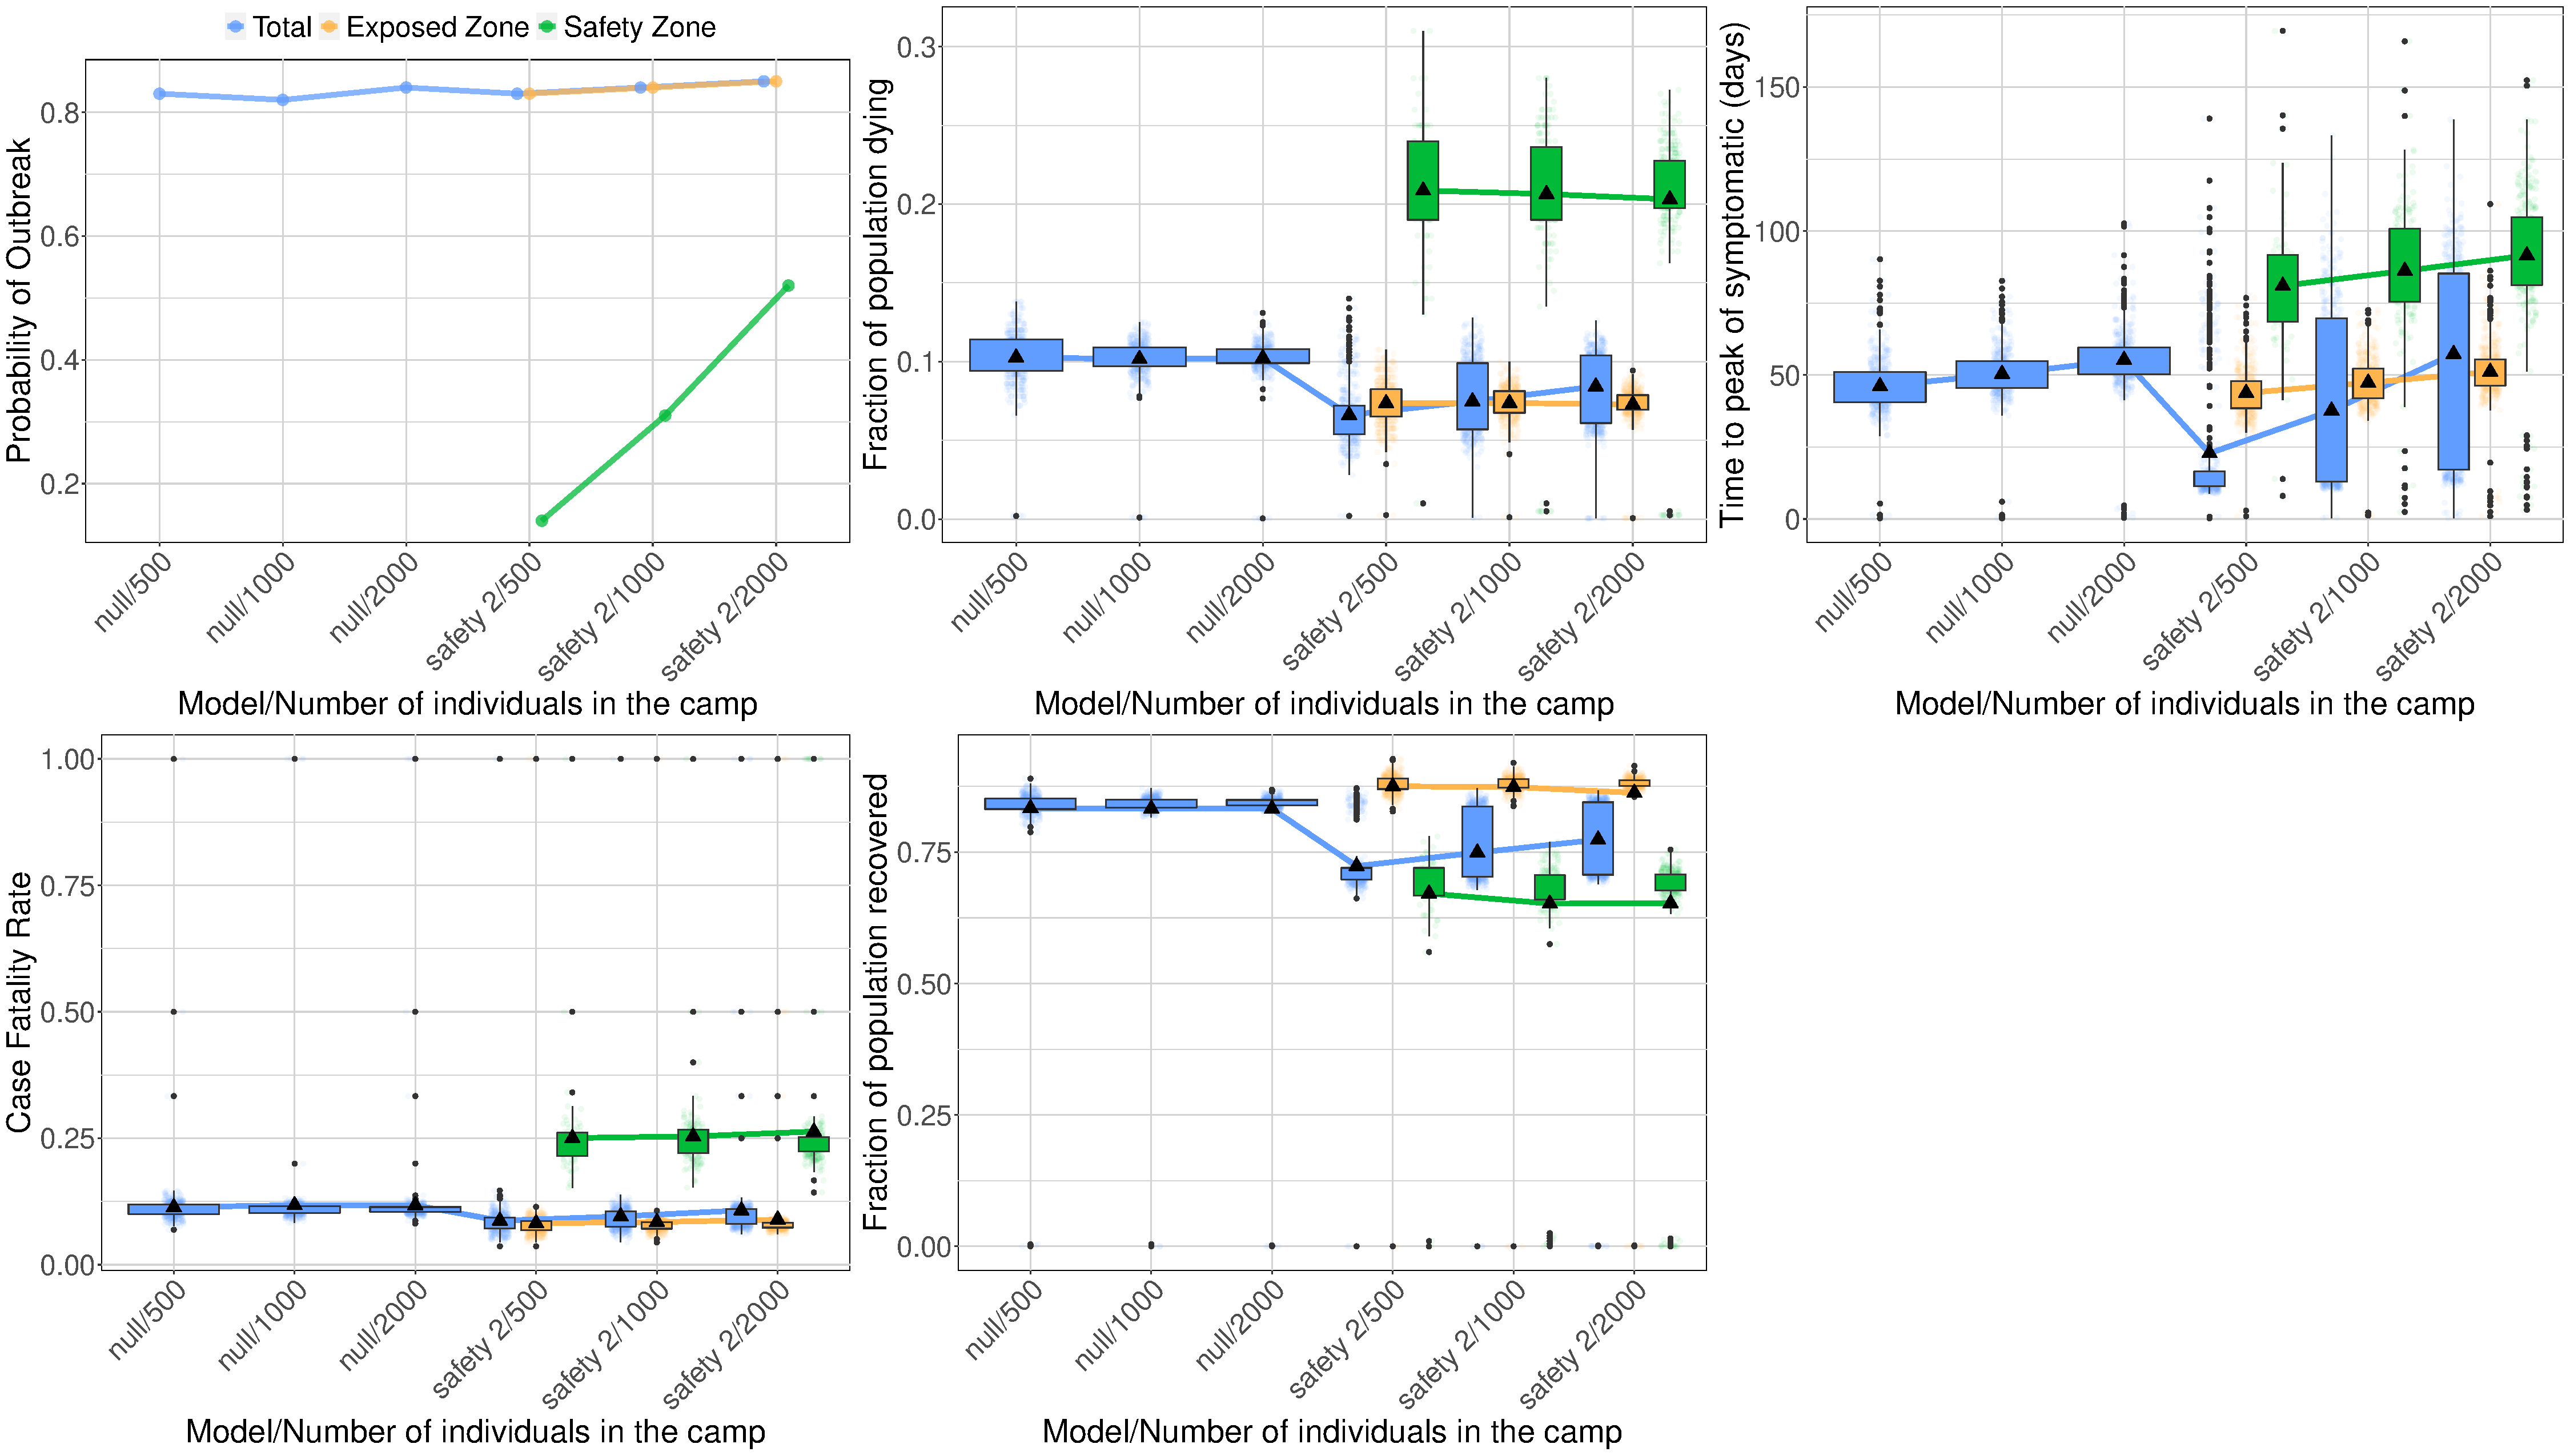
\includegraphics[width=1\textwidth]{figures/FigS10}\hspace{2mm}
\par\end{centering}
\caption{\label{fig:Suppl_popClass} \textbf{Population moving to the safety
zone.} Probability of an outbreak (top left), fraction of the population
dying (top middle), time until peak symptomatic cases (top right),
IFR (bottom left), and fraction of the population that recovers (bottom
middle) as a function of the safety zone allocation scenario (see
Table \ref{tab:SafetyScenarios}). All figures consider the scenario
with 2 contacts in the buffer per person in the safety zone per week.}
\end{figure}
\medskip{}

\begin{figure}[H]
\begin{centering}
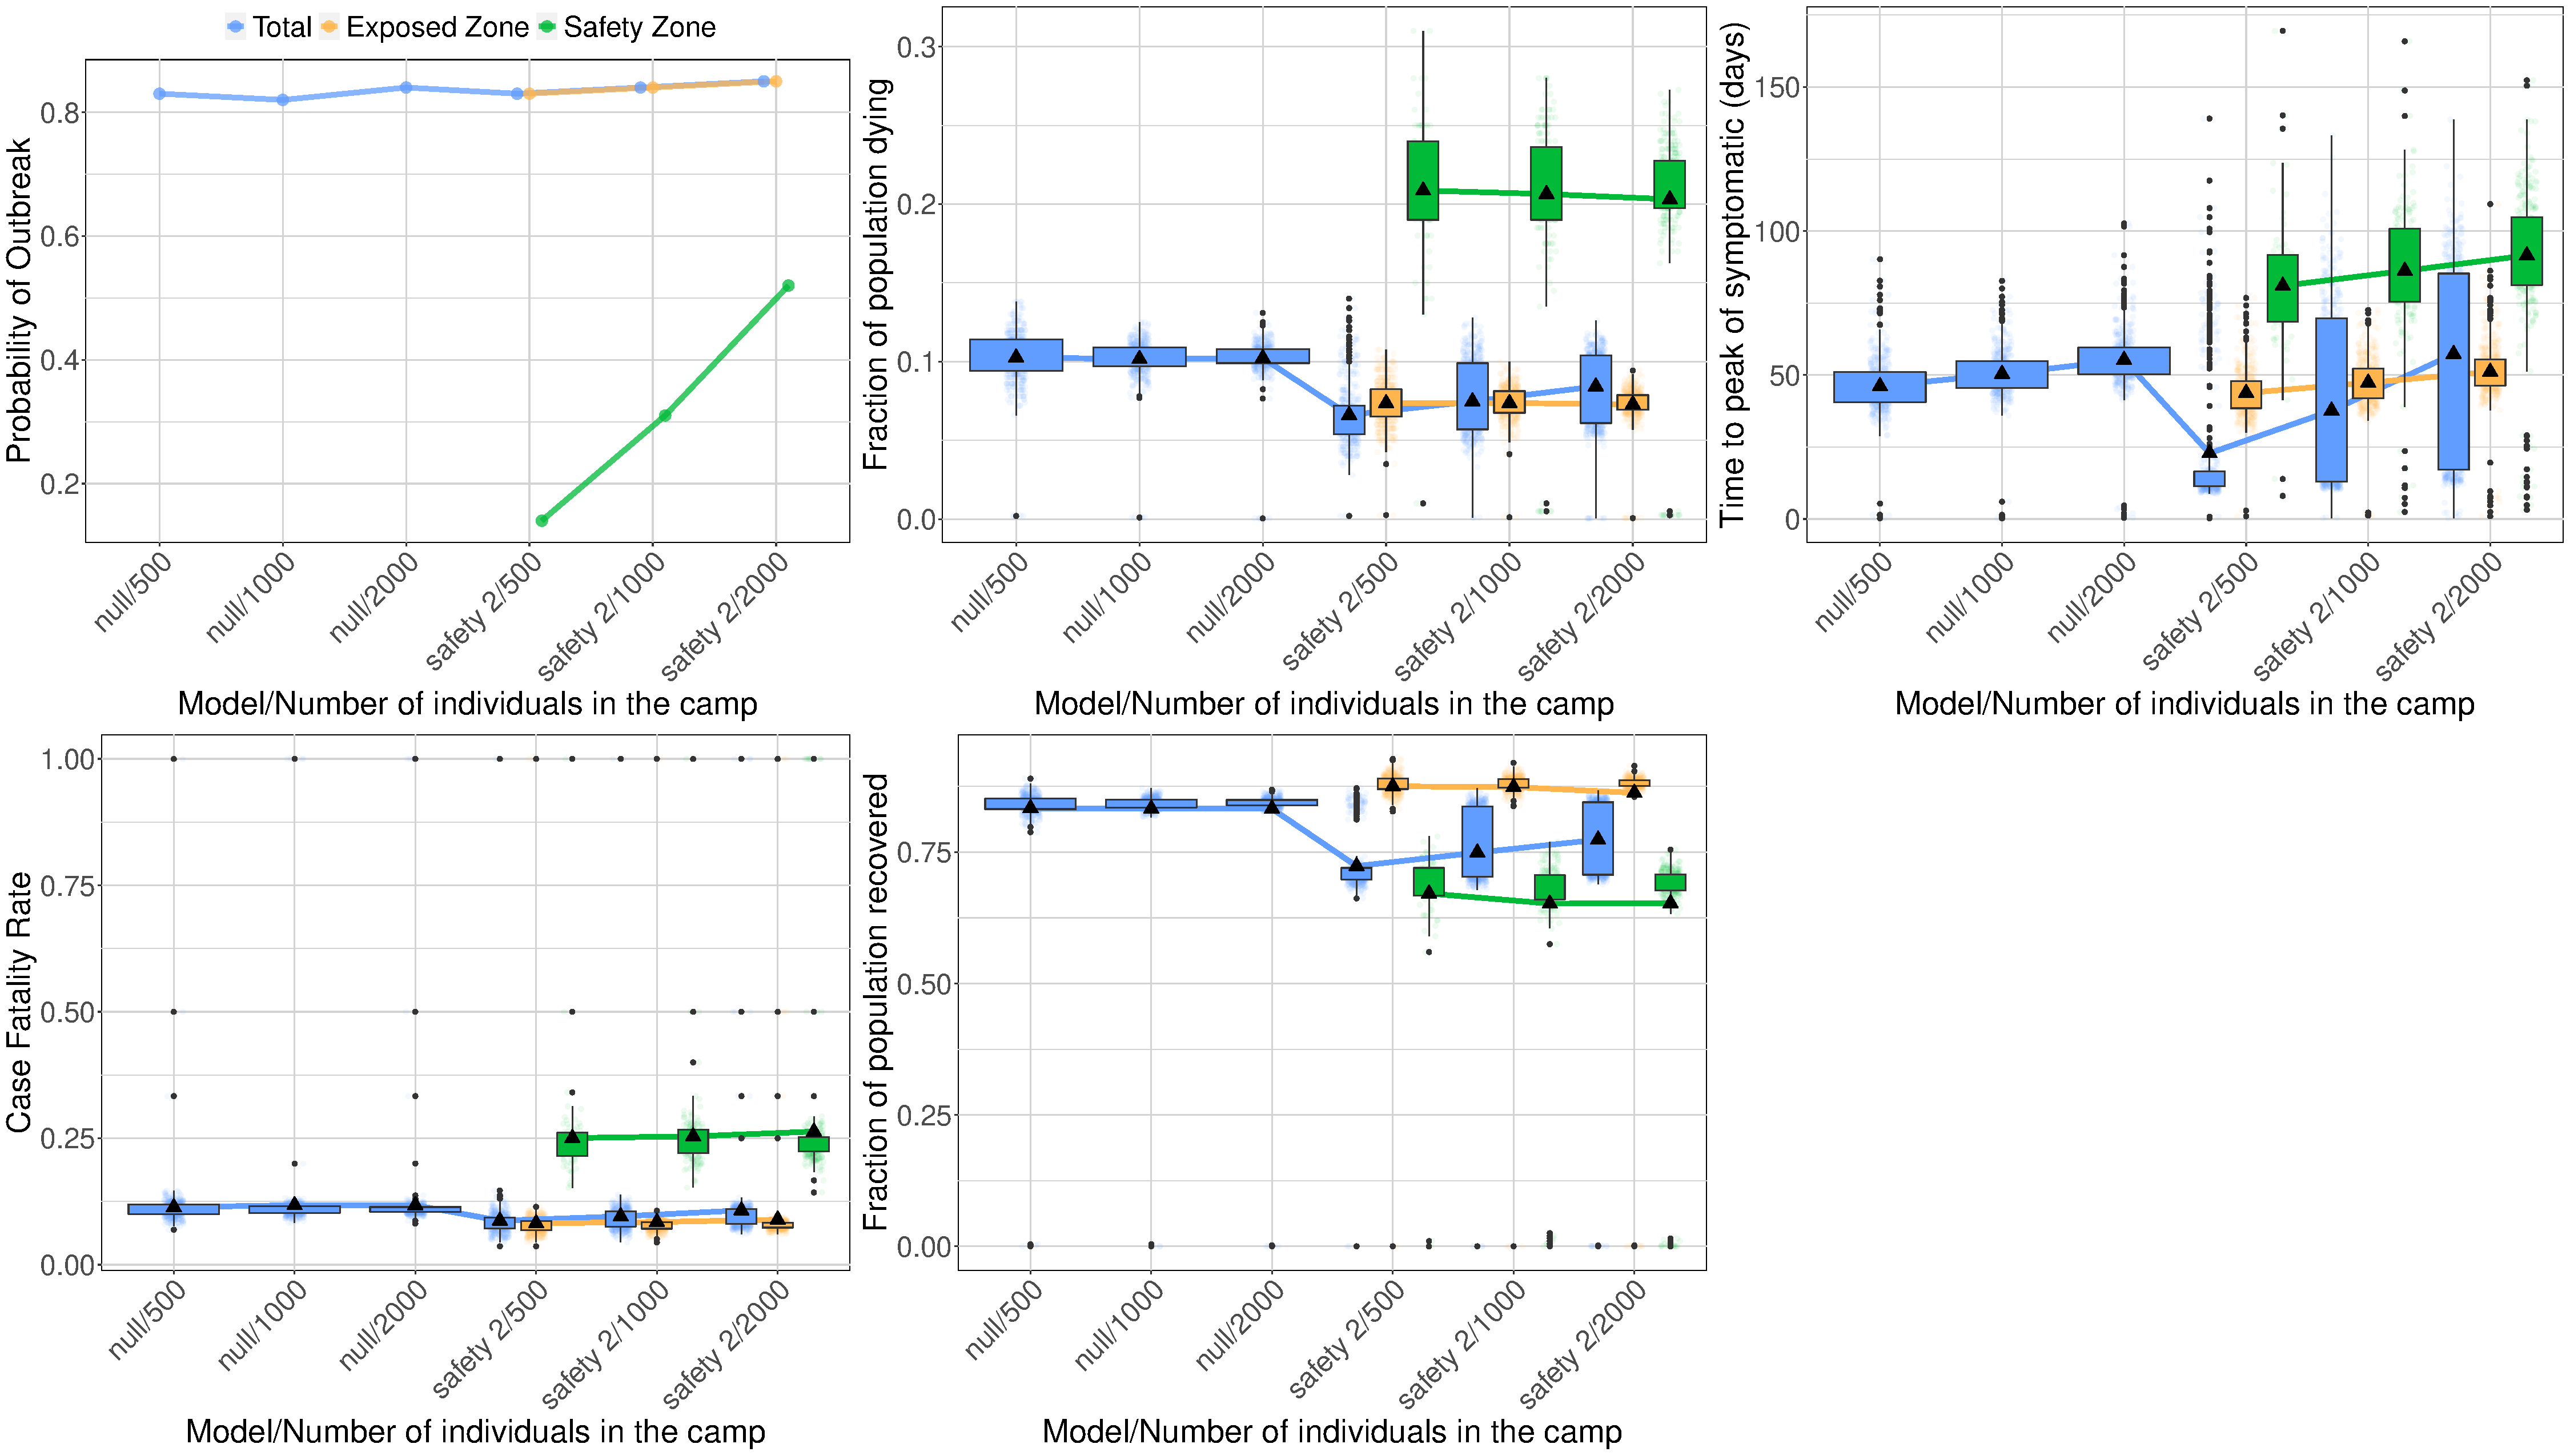
\includegraphics[width=1\textwidth]{figures/FigS11}\hspace{2mm}
\par\end{centering}
\caption{\label{fig:Suppl_popSize} \textbf{Efficacy of the safety zone for
different population sizes.} Probability of an outbreak (top left),
fraction of the population dying (top middle), time until peak symptomatic
cases (top right), IFR (bottom left), and fraction of the population
that recovers (bottom middle) as a function of the total population
size. The figures consider scenarios with no interventions (null),
and with a safety zone comprising 20\% of the camp's population with
2 contacts in the buffer zone per person in the safety zone per week
(safety 2).}
\end{figure}

\medskip{}

\begin{figure}[H]
\begin{centering}
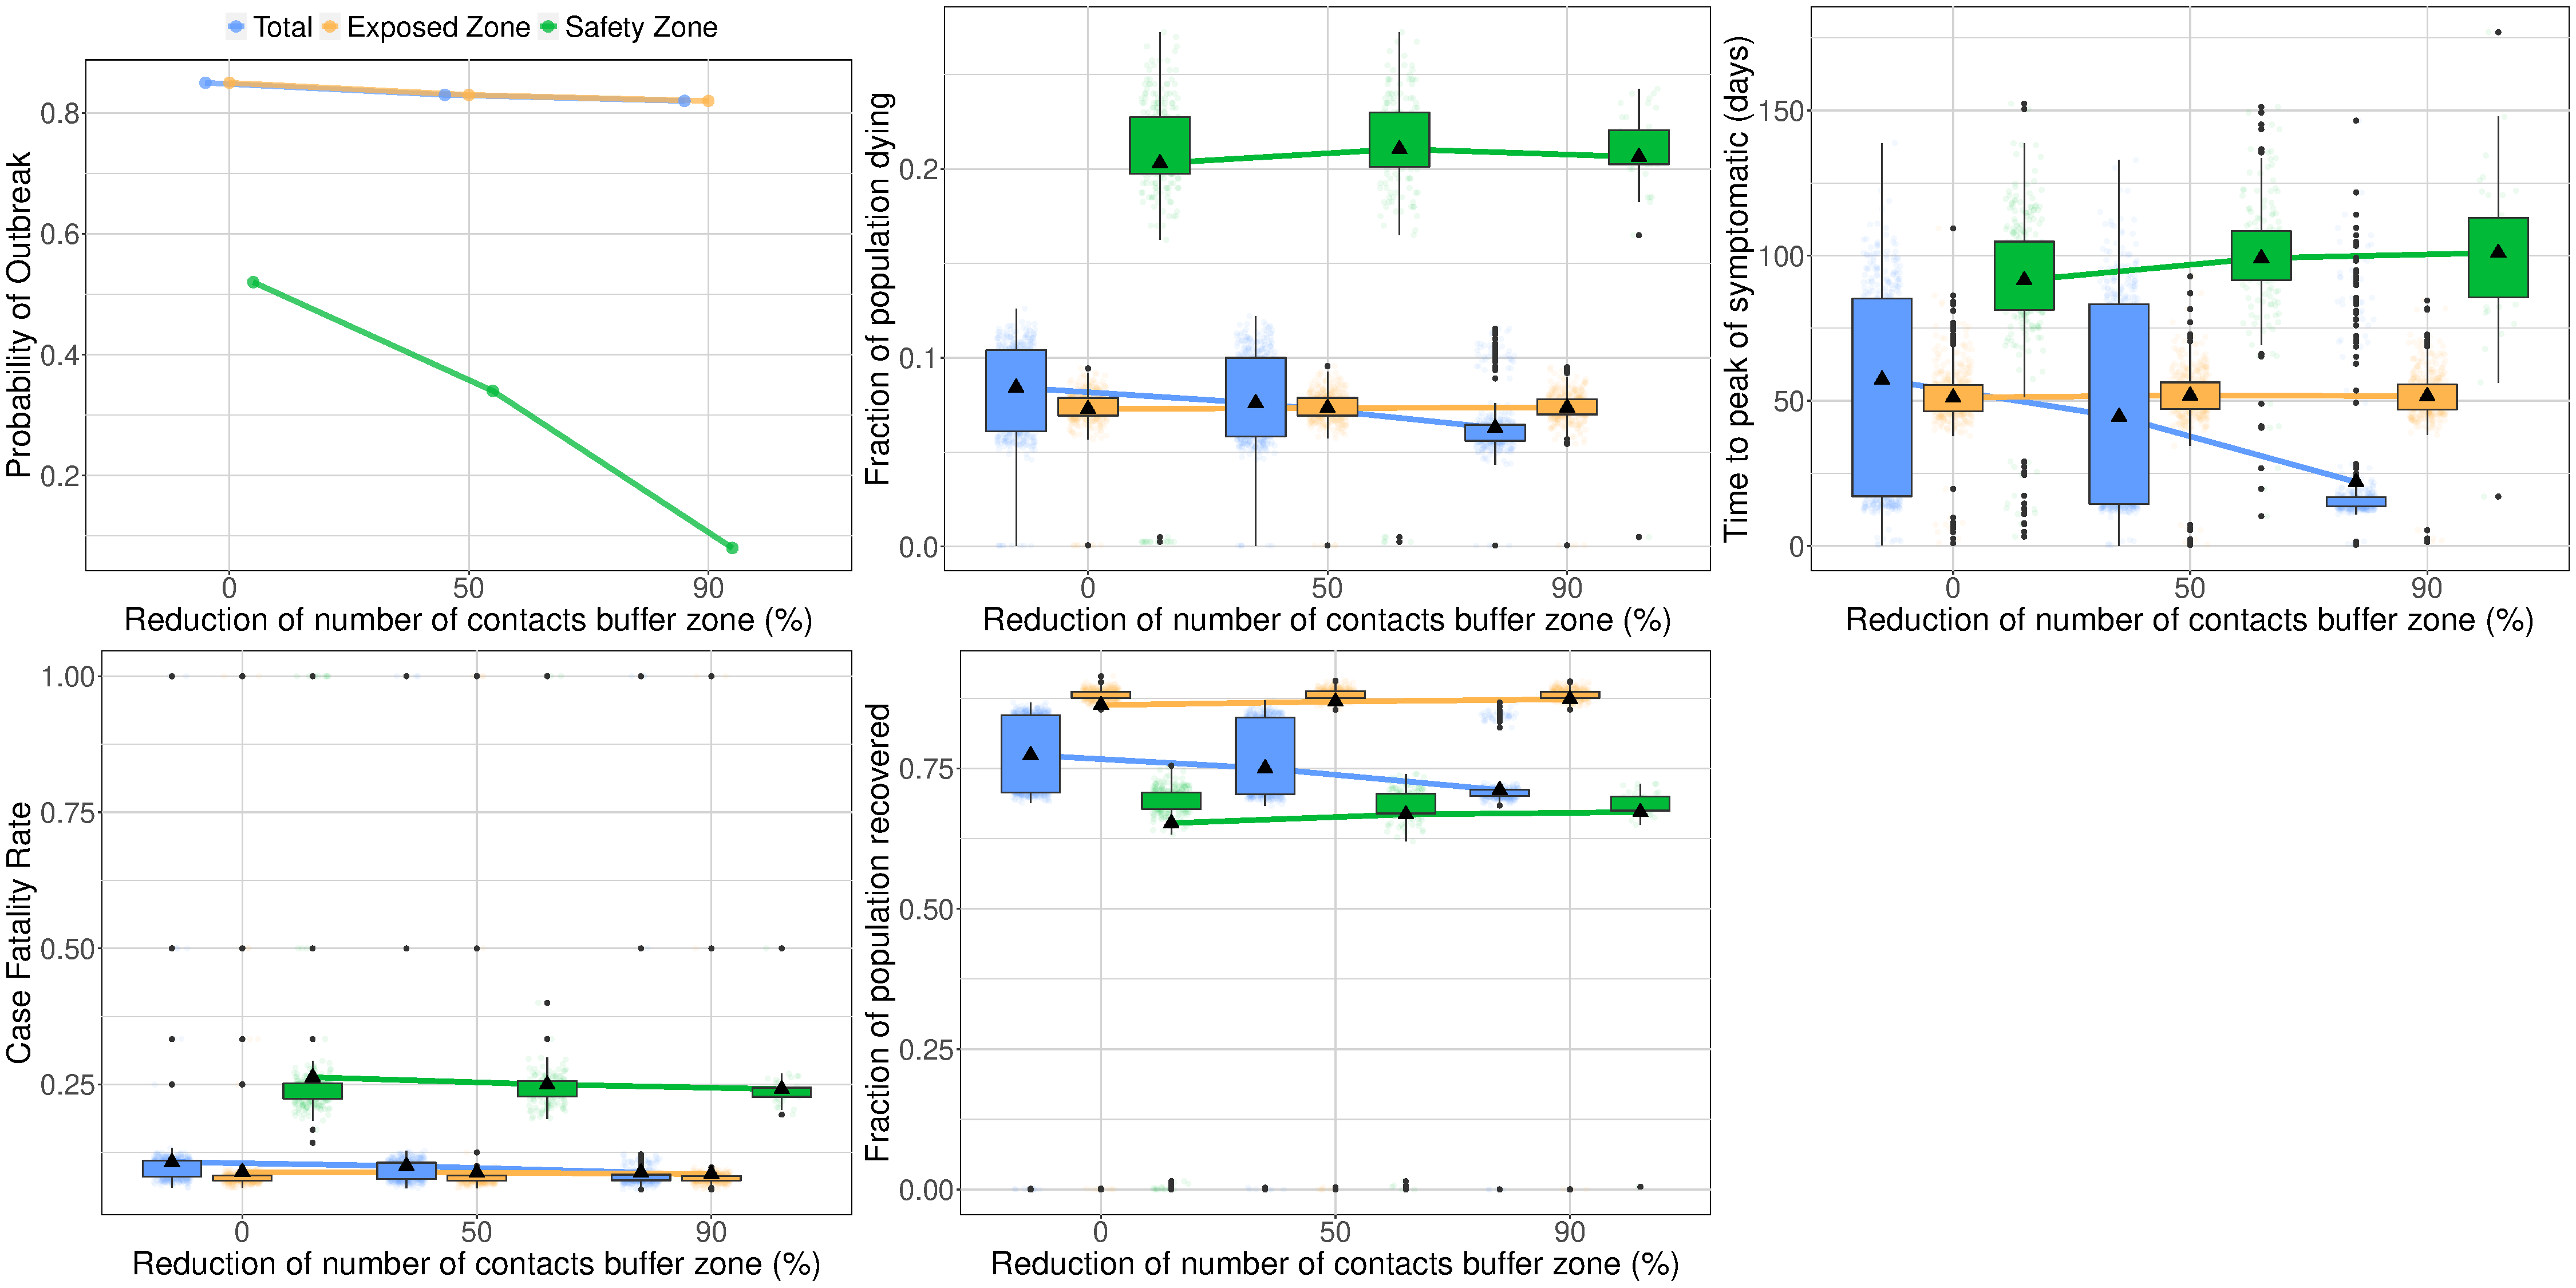
\includegraphics[width=1\textwidth]{figures/FigS12}\hspace{2mm}
\par\end{centering}
\caption{\label{fig:Suppl_lockdown} \textbf{Lockdown of the safety zone.}
Probability of an outbreak (top left), fraction of the population
dying (top middle), time until peak symptomatic cases (top right),
IFR (bottom left), and fraction of the population that recovers (bottom
middle) as a function of the reduction in the number of contacts permitted
in the buffer zone from a baseline of 2 per person in the safety zone
per week. All figures consider the scenario in which 20\% of the camp's
population is allocated to the safety zone.}
\end{figure}

\medskip{}

\begin{figure}[H]
\centering{}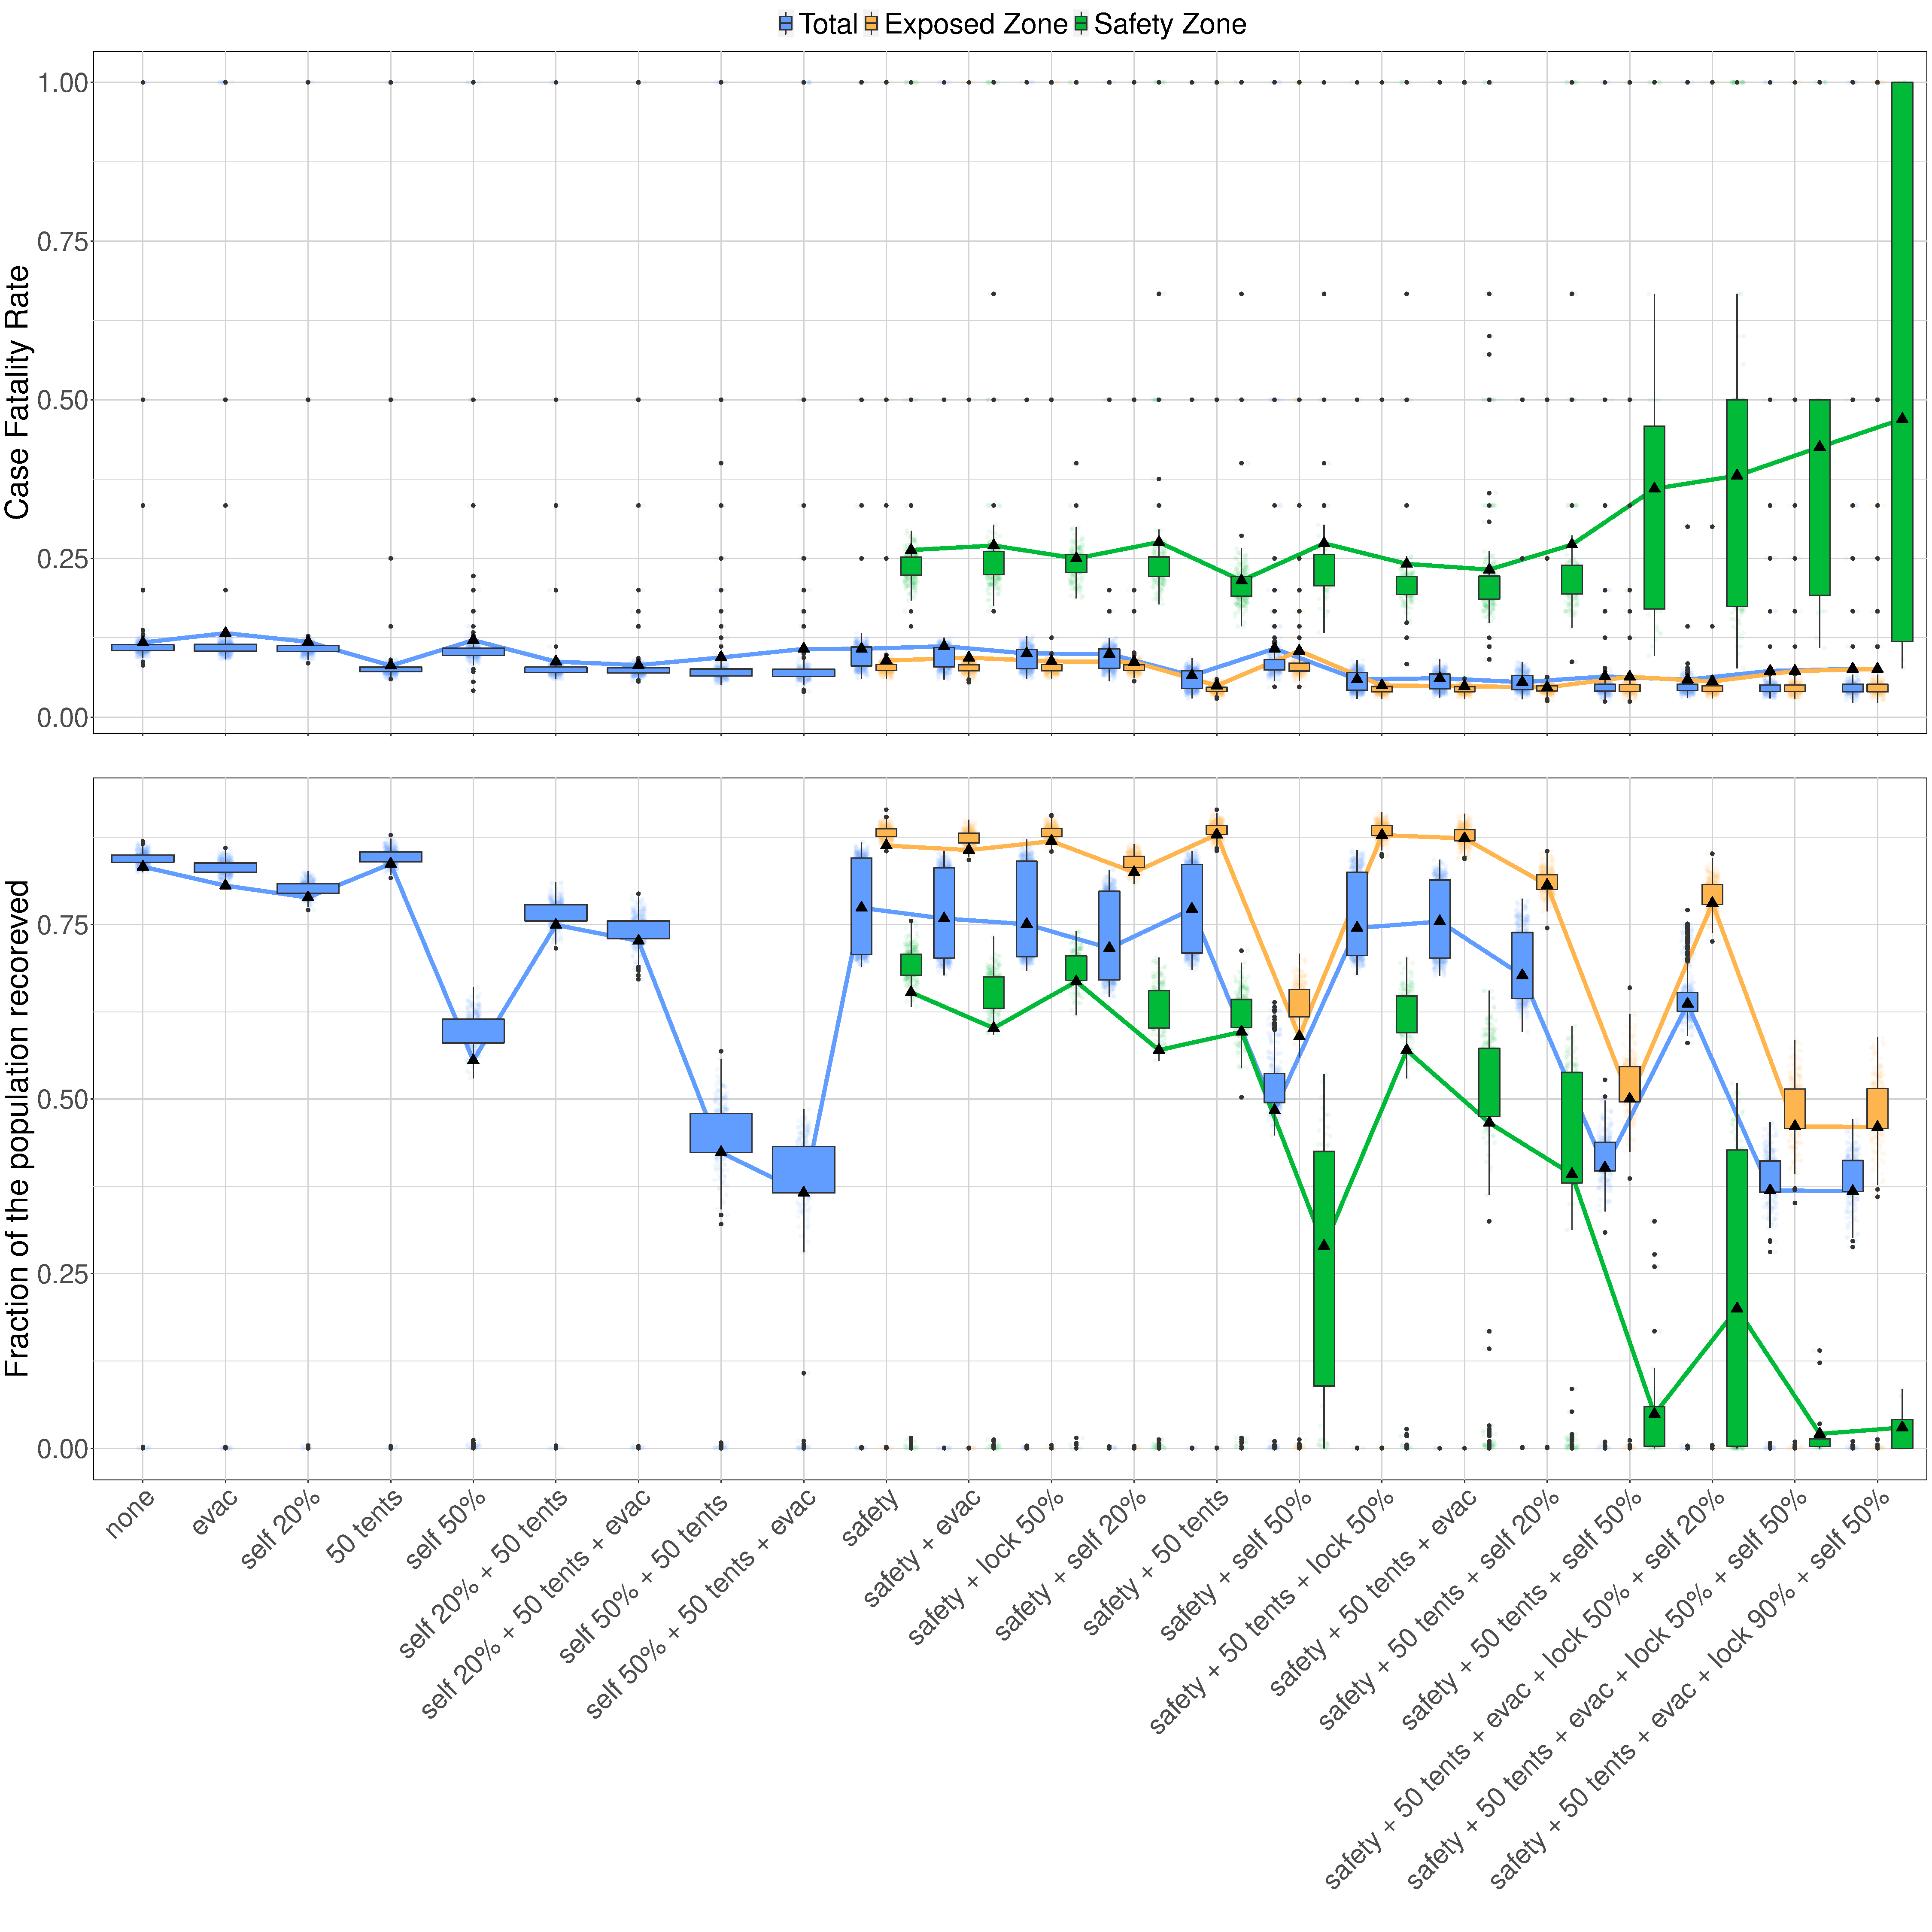
\includegraphics[width=1\textwidth]{figures/Fig_S13}\hspace{2mm}\caption{\label{fig:Suppl_combined} \textbf{Combined interventions.} IFR (top),
and fraction of the population that recovers (bottom) for different
combinations of interventions. Evac = evacuation of severely symptomatic,
self = self-distancing, tents = number of available self-isolation
tents, safety = safety zone, lock = lockdown of the buffer zone. For
combinations of interventions including a safety zone, we distinguish
between the population living in the green zone, in the orange zone
and the whole population. The increase in the IFR for the green zone
is explained by the discretization of the possible values that the
IFR can take when the number of cases is very low (see Supplementary
Table \ref{tab:CFR_discrete}).}
\end{figure}

\begin{table}[H]
\begin{centering}
\includegraphics{figures/Table_S4}
\par\end{centering}
\caption{\label{tab:CFR_discrete} \textbf{Efficacy of the safety zone in combination
with other interventions.} \textless 20 cases = number of outbreaks
in the green zone with fewer than 20 cases recorded. Total = total
number of simulations where an outbreak in the green zone occurs (at
least one death). \% of total = percent of outbreaks where fewer than
20 cases are recorded. N = 500 simulations for each combination of
interventions. For the most effective combinations, the majority of
simulations where an outbreak occurs in the green zone see fewer than
20 cases. In these simulations, the discretization of the possible
values that the IFR can take explains its apparently anomalous increase
in Fig. \ref{fig:Suppl_combined}.}
\end{table}

\newpage{}

\bibliographystyle{unsrt}
\bibliography{req550-syria}

\end{document}
